\chapter[南粤史纲要]{南粤史纲要\protect\daggerfootnote{本文为2015年11月8日冬川豆组织部分南粤豆粉集体学习南粤历史时,执经生的录音整理稿。全文共计4万6千字,2016年2月4日~10日之间分5篇首发于冬川豆。感謝場記三马兄,并向阿姨、硕帝致敬。}}

\footnotetext{注:“阿姨”指刘仲敬,当代诸夏独立理论奠基人,2018年11月起任大蜀民国临时总统;“硕帝”指李硕,自称“满洲国皇帝”,时常编写文章支持满洲国独立,后来投共。}


\begin{quoted}这些南越人跑到丛林里,宁可跟野兽待在一起也不肯作秦朝的降虏。\end{quoted}

\section{前言}
我今天讲南粤史。南粤史一个特点就是要以南粤为本位去讲这段历史。因为我们从小到大接受的历史教育都是中国的王朝史观,看南粤就是从首都的角度去看地方的历史,这是一个很扭曲的图景。既然讲南粤史,就要以南粤为本位。这是我要讲的它的第一个原则。第二个原则就是,我不会太关注那种技术性的东西,比如说什么时候发明了一个瓷器,什么时候造出一个很NB的发明等等,这些东西其实相对来讲都是技术上的枝节问题。还是要按照阿姨说的,我们要以路径、节点去看这段历史。最重要的就是宪制——权力的关系还有族群之间的关系。这就是我要讲的两个原则,我们把握南粤史要以这个为脉络去把握。首先就要看一下地图,这个就是南粤史的舞台:

\begin{figure}
	\centering
	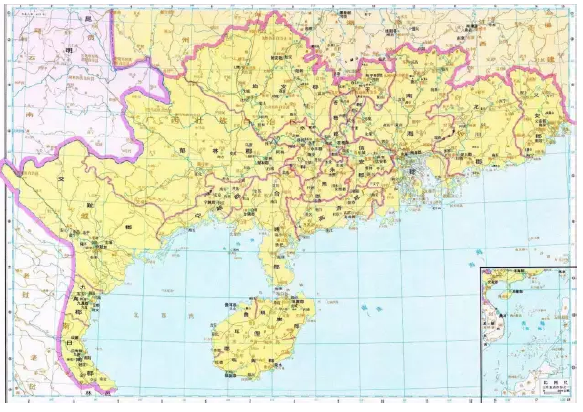
\includegraphics[width=\textwidth]{images/image-3}
	\caption{岭南}
\end{figure}

首先我们就要给南粤下一个定义。我个人的定义首先当然是五岭(越城岭、都庞岭、萌渚岭、骑田岭、大庾岭)以南;第二,它跟今天的广东省不完全重合,它还包括广西东南这一块今天叫做北海的地方。再往西的话,广西的整个东南部也可以算作南粤的一部分,它也是白话(粤语)人群的地方。大致上来讲还是跟今天广东的重合度蛮高的。这个地理区域有一个特点:它地理上有封闭性。它对北边是封闭的,对南边是开放的,南边是海。

在20世纪粤汉铁路通车之前,你从湖南到广东是很难的,粤湘之间的骑田岭道路非常崎岖。一般来讲,北人南下或者粤人北上走哪些路呢?主要是三条路:第一条路就是沿着西江上去,走灵渠,再往上到北方,走水路;第二条是走大庾岭,再往上面走就是赣南山区;第三条路就是跟闽南联通。大概是这样的三条路。这三条路都不是太好走的。因为首先,珠江水系就是比较封闭的,你要从北方进入,秦朝还非得凿一个灵渠你才能过去。大庾岭其实也不是那么好翻的。东边也山地众多,比较难走。所以整个的地理环境是构成了一个地理单元,能够让它有条件形成比较独特的文化。

\begin{figure}
	\centering
	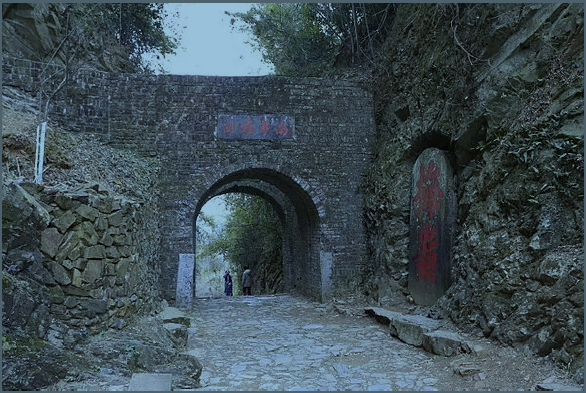
\includegraphics[width=\textwidth]{images/image-1}
	\caption{梅关关楼北面门额刻“南粤雄关”,北侧石碑上刻“梅岭”}
\end{figure}


我们整个来看南粤的话可以分成三块地方,以三个地方为中心。第一个就是我们所待的珠三角。这一块的地形特点就是,有比较大的肥沃的平原。在珠江口的西岸,今天中山、珠海、澳门这些地方,它的土地是很碎的,这些也大概是宋代以后才形成的,是珠江带来的沙冲积出来的平地,这些地方开垦出来的田地叫做沙田。这一块地方是非常富庶的,它的灌溉也很容易。这个地方又处于一个地理位置的中央,我们可以把它看成南粤的中心。它的中心城市就是广州。这就是南粤最大的一个中心。

还有一片非常富庶的平原就是韩江流域。这个地方有一座大城市,潮州。韩江流域的开发要相对晚一些,要到唐宋之后才开始有所开发。这块地方也是很富庶的。它因为跟福建比较近,它受到闽文化影响非常大,最后在这个地方形成了潮汕民系。

还有一块比较大的区域,就是东北部的山区,它靠近江西。这块地方的特点就是,它相对的比较贫瘠。而这个地方也形成了一个群体,也就是客家人。清朝是专门划了一个地方叫嘉应州,在潮州的北面,这个地方就是今天的梅州,这个地方就是客家人的中心。大概在明清之际的时候,客家人从这个地方往西一直到珠三角,最后形成了今天这个三大民系的格局。

\begin{figure}
	\centering
	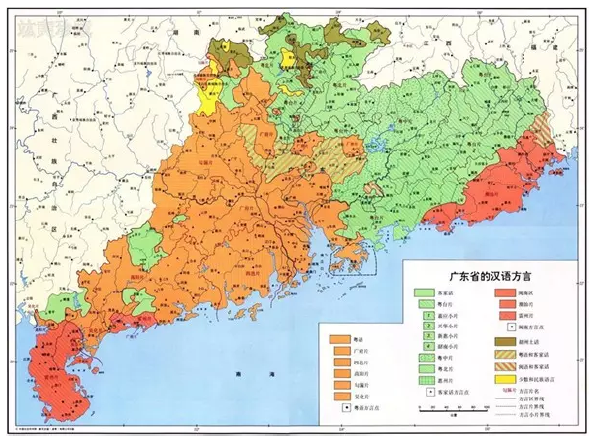
\includegraphics[width=\textwidth]{images/image-2}
	\caption{南粤方言分布,其中橙色为粤语,绿色为客家话,红色为潮州话。}
\end{figure}

我们把握南粤历史就要先知道有这三块区域。最大的、最重要的中心,当之无愧的就是珠三角这一块。还要提醒的是,闽人拓殖到韩江流域,接着他们一直沿着海岸线西进,在唐宋以后,雷州半岛还有海南岛也是讲闽语的人所覆盖的,他们跟潮汕人是有亲缘关系的。这大概就是三族的地理分布。大概讲了这个背景之后,我们就进入正题。

既然要以南粤为主体去讲南粤史,肯定就不能按照中国的王朝划分去讲南粤史的时期了。于是我借用了越南史的一个概念,就是“自立”和“北属”。越南人写他们的历史:它被中国统治的时候,他就叫这个时期“北属时期”;它自己自立的时候,他就叫做什么什么朝。南粤史也是这样的,它是不断地有自立的政权出现,又不断地有北属的时期,这样一个个间隔开来的。而它跟越南不太一样的是:越南在宋代以后基本上就完全脱离了中国了;但是南粤的历史大部分时间还是被帝国所占领的。南粤史,大家看我讲完之后就会知道:历史上是有四个自立政权的,分别是南越国、冼氏政权、南汉国、何真政权;以这四个为间隔点,于是就出现五个北属时期,就是第一次到第五次北属。我是这样划分南粤历史的。

\section{南粤史前史}


首先讲一讲史前史。在史前的时代,我们就能看到后来所谓三大民系的三大版块已经出现端倪了。大概在三千年到六千年前,首先是韩江流域和珠三角流域,就是今天广府人和潮汕人的地方,就出现了大量的贝丘遗址。“贝丘”就是大量贝壳的堆积层。这些人捕捞贝类,然后拿去食用,是这样一些住在海边的人。这些人未必是掌握了什么农耕技术,他们的蛋白质摄入量应该相对高一些,是一种初民的德性。而粤东北的山区,就是客家人待的那个地方,当时就出现了农耕的文明,因为它的自然资源可能相对没有那么丰富,他只好去种地,然后就出现了稻作的文明。

当时整个南越的文明有一个特点,就是它的石器、陶器跟玉器非常的漂亮,而且跟吴越的良渚文化非常近似。所以说其实当时是存在一个泛百越民族的,南越就属于那一块的。这个文明大概持续了三千年左右。到了三千年前,进入了青铜时代。这就涉及到这些人是什么人了。这些人是百越。百越是一个概念,因为在华夏人看来,当时整个东南沿海这些地方都是越人的地盘。当然越人是分成好多好多种的,百越就指非常多种越人。他们跟华夏族不是一个种族。他们说的话可能跟今天的泰、缅语比较相似,跟汉语其实是没有太多关系的,不像今天的粤语毕竟跟汉语还是有很大的关系的。他们跟今天的广东人还是不一样的。

\begin{figure}
	\centering
	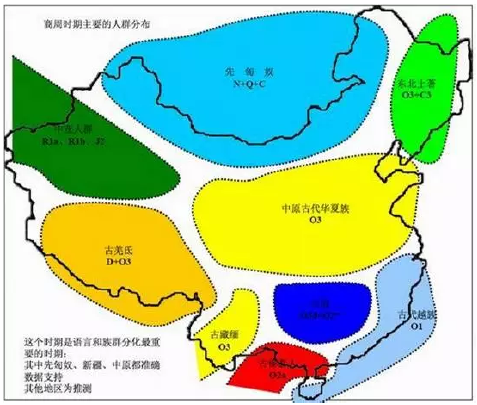
\includegraphics[width=\textwidth]{images/image-4}
	\caption{商周时期诸夏地区主要族群y染色体分布}
\end{figure}

我们可以从分子人类学的证据来看到,其实今天的广东人还有很多O1的染色体,虽然可能没有O3多,但这个是非常大的一个比例,因为我们也不知道严实到底对他这个数字有没有做手脚,严实说O3比O1要多一些,但是O1也很多。不管怎么说,百越的血统今天依然在南粤人的血统当中发挥了很大的影响。这个是史前人种的问题。

\section{百越时代}

接下来,我们可以看到三千年前左右,也就是公元前一千年左右,这个时候大概是商周之际,百越人开始出现在了华夏所记载的典籍当中。大家应该读过《经与史》,阿姨说过,上古的诸夏一直到商代,跟百越有一个最明显的不同:北方的各邦打起仗来非常的残酷,而它的文明程度相对比较低,它的物质丰富程度跟器物的精致程度远远不如南方百越这些人;而百越的一个特点是,它的物资丰富程度高,生活非常的精致,但是它的战斗力并不是很行,它并不是以军事为主导的文明,它互相杀戮的战争的规模也不是很大。我们从它的遗迹中那些出土的骨头就能看出来:如果有夏朝的话,夏商时代的这种骨头,有的人真的是被cut into slices,被剁碎了,可能直接跟动物骨头一起混着被人吃掉了;而南方看到的这些被打死的人,可能基本上一两下就被打死了,可能就是战争中大家随便打一打,然后不小心误伤打死了几个人。他们主要的生活不是战争,而是宗教和丰富的物质生活。相对来说,它的组织度肯定是没有北方高的。而北方的组织度似乎是高一些,有组织比较严密的军队,有文字,我们现在用的文字是从北方这个系统下来的。

首先我们能看到的是北方对南方人群的记载——我们看不到南方对北方华夏的记载,所以这时候只好用北方的记载——首先就是据说在周武王的时候,他把南越这一块地方叫做“扬越”,说南越是“扬州之末土”。我们知道,据说夏禹时代分天下为九州,扬州就是今天吴越那一块。对周武王时代的人来讲,扬州再往南那个地方就像今天玩游戏的战争迷雾一样,他也说不清楚,那个地方就是迷雾,也说不清楚是什么。那里可能也属于扬越,属于扬越不太入流的一支。所以我那个歌(见下),叫“扬越之苗裔”,就是这样来的。因为他们又在扬越的南部,所以又叫“南越”。而“越”和“粤”是通的,所以也叫“南粤”。国名就是这样来的。

\begin{quoted}
	歌名:《南海波涛》\\
	词:执经生\\
	南海波涛、南岭雄豪,神佑我南粤之疆土。\\
	木棉花开,珠江滔滔。卫我家邦,唯我同袍。\\
	扬越之苗裔,华夏之嫡传,二千年历史,决断在今朝。\\
	众志成城,一心一力,洪水漫天,同胞怒号。\\
	众志成城,一心一力,洪水漫天,同胞怒号。
\end{quoted}

\begin{figure}
	\centering
	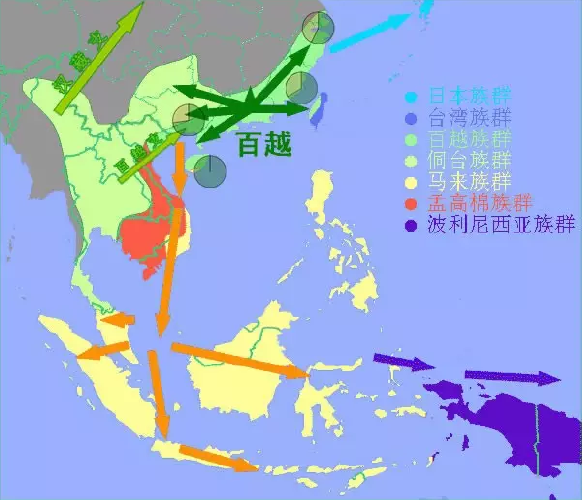
\includegraphics[width=\textwidth]{images/image-5}
	\caption{百越语族现今的分布范围及对百越发生和分化的猜测。}
\end{figure}

再到后面就是《礼记》——其实我们也不知道《礼记》是不是有汉代人动过手脚——它就说南方有一种蛮,这些人有一个什么特点呢?他们“雕题交趾”。“雕”就是刻,“题”是额头,就是说他们在额头上会画纹身;“交趾”,说他们的大脚趾是分开的,反正跟中原人不一样,他的两只脚并拢在一起的时候,大脚趾会交在一起,反正是一种很奇怪的人。而且说他们“不火食”,就是不会吃熟食。还有一个就是《山海经》,“其为人人面有翼,鸟喙。”说岭南这个地方的人很奇怪,他们人人长着翅膀,有鸟嘴。其实它说的这个是事实么?这不是事实。但是这个反映出当时的一种观念,就是说对于华夏族来说,这些地方的人就是相当于野兽一样,就是加了一些很荒诞不经的想象,这些人跟自己完全不是一回事。

再后来,慢慢的我们就能看到,北方的有组织度的文明第一次进入了南越。这个就跟战国时代的楚国有关系。我们知道越国在春秋末期很厉害,它把吴国打败了,然后它一直北上,当过老大。但是到了战国的时候,它不行了。然后,楚威王在公元前306年把越国灭掉,把越国的国王无彊给杀掉了。据说无彊的儿子叫之侯,他就跑到了岭南自立为君。这个大概是我们能看到的历史上第一次,南粤出现像君权一样的东西。而这个君权不是本土产生的,而是北边的越国来的。当然越国人也是百越,可能种族上比较相近。

当时,在史书的记载中,出现了两个本土的人。一个叫做公师隅,据说之侯派公师隅到北方去联络魏国,让魏国牵制楚国。我们就可以看到,很有可能之侯到了南越本地之后就本地化了,他用的都是本地的这些人。据说公师隅筑了一个城叫南武城,这个城就是今天的广州,所以广州建城是非常早的,大概2300年前。还有一个人,这个是比较确定的,这个人叫高固,他也是南越人。这个人对华夏这一套文化很熟悉,他熟读《左传》,当时他跑到楚国去入仕。我们知道春秋战国这些游士是到处乱走的,这个人其实也是个游士。说楚威王读不懂《左传》,他就帮楚威王做宰相,帮他读《左传》。我们也可以看到当时华夏的影响已经对南粤很大了,已经有人开始读华夏的东西了。这个是战国时代。

当时南越族的习俗,我们能从今天的广东人身上看到很多东西。中原人觉得这些人就是像野兽一样不可思议的,虽然有那么一两个可以被理解的,比如说高固,这种人是游士。他们描述的南越人就是这样的,首先,他吃的东西跟华夏不一样:华夏主要就是吃肉,吃鱼也是河鱼;但这些人吃海鱼,吃鳖,还有吃蛇。今天广东人也是这样。第二个,他们不住屋子,他们住“巢”。其实不是巢,而叫“干阑”,今天我们在东南亚能看到很多干阑式的建筑。因为这个地方太潮了,一楼是不能住人的,于是当地人就在地上架起架子,有一个梯子爬上去,在上面住人,这样的一个房子。在中原人看来,这个东西是个什么呢?就是个“巢”,所以说就觉得很奇怪,这些人简直难以理解。

\begin{figure}
	\centering
	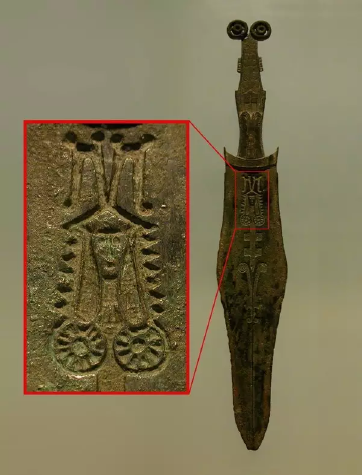
\includegraphics[width=\textwidth]{images/image-6}
	\caption{雒越人首纹青铜匕首}
\end{figure}

第三个是,这些人跟华夏族完全不一样:我们知道华夏族是束发的,一直到明朝都是束发的,搞一个发髻在上面;在华夏族看来,这些南越人不束发,居然不相信身体发肤受之父母,他们剪头发的,断发的,而且他们还在身上纹上奇怪的花纹,这些人太奇怪了,不能理解。而且这些人的发型也跟华夏不一样:华夏是在上面一个大髻;他们是在后面搞椎髻,把头发拢到后面去。而且华夏诸邦,我们知道《周礼》的世界,阿姨也写过,他们是不太像商人那样相信巫鬼的;而这个时候南越人是相信这些神神怪怪的巫鬼的。我们现在当然可以说这是一种原始德性的体现,但华夏族也不太能理解。

第四个就是,这些人不用战车,他们打仗是划船的,打水战,因为这个地方水多。第五个是这些人没有君主。我们之前看到有之侯,但之侯后面有谁,我们不知道了,又没了。当时南粤的政治组织度不强。大概在当时的中原人看来,这就是一个很异类的社会,而且它的政治组织度是不如中原的。等于是除了它出了几个像高固这种游士以外,基本上它跟中原没有太大的关系。这个就是百越时代。


\section{粤秦战争、首次北属}

这种情况到了秦政开始之后就完全变了,就是粤秦战争和南粤的第一次北属。我们知道公元前221年秦始皇统一了六国,他接着就北击匈奴,当然搞了各种各样丧心病狂的事情,什么修长城、给自己修陵。北击匈奴,南伐南越。公元前215年,经过六年的准备,他派蒙恬带三十万人北击匈奴。一年后他接着再派一个将军,叫屠睢,带兵攻打南越。你看他派的兵都是些什么人:逋亡人是什么人呢,“逋”就是逃,比如说逃兵役、逃税的这些人再给他抓回来的这种流民;还有赘婿,赘婿在周礼的封建社会地位高么,不高的;还有贾人,就是做买卖的人,他们的共同体的属性并不是那么的强、流动性相对大,也受到秦政的歧视。可以说他用的都是相对没有组织度的人,这些人打起仗来不要命,反正他们也几乎一无所有。秦始皇就让他们去打南越。

这些人初次进军非常的顺利,当年就打进去建了三个殖民点:一个是“桂林”,不是今天的桂林,但郡治还是在今天的广西境内;一个是“南海”,就是广州,就是公师隅的广州;还有一个是“象郡”,是在今天越南的北部、广西西部和南部。一年基本上就殖民完了。他们是怎么来的呢?兵分五路,从北面大举南下。接着他们就sb了。他们发现很不好打,他们进去之后就进入到了百越人的人民战争的汪洋大海当中。这些人在孤立的殖民点里面,后勤根本也跟不上,秦始皇就不得不凿了灵渠去补给他们,大家知道灵渠是连通西江跟湘江的,因为用水,他运补给比较快。

\begin{figure}
	\centering
	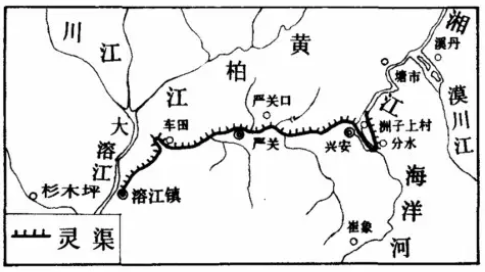
\includegraphics[width=\textwidth]{images/image-7}
	\caption{灵渠地图}
\end{figure}

这个时候,可以看到《史记》里面的记载,说南越人当中出现了一个人叫“西呕君译吁宋”,西呕是南越的一个部族。似乎这个时候因为秦人的刺激,这边也出现了一个君,就是说在北方的强权的刺激之下,这边的组织度被迫凝结起来,也出现了一个君。然后他跟秦人打仗,就被杀掉了。这之后,就是非常伟大的一幕,南越人“皆入丛薄中,与禽兽处,莫肯为秦虏”。这些南越人就跑到丛林里,宁可跟野兽待在一起也不肯做秦朝的降虏。最后打了三年。秦军是“三年不解甲弛弩”,疲于奔波。最后是南越人“夜攻秦人,大破之,杀尉屠睢,伏尸流血数十万”,不光杀了秦军主将,还给秦军造成了非常惨重的损失。这是一场非常伟大的胜利,南粤历史上第一场抗击外敌的伟大胜利。

屠睢挂掉了之后,秦朝派另一个叫任嚣的将军取代他。屠睢的副将赵佗——就是后来的南越武帝,依然担任军队二把手。秦就改变了策略,明白不能光派军队下去,要派大规模的殖民者到南粤去。于是“以谪徙民五十万戍五岭”,其实也就是这种亚述式的大迁徙,翻过了五岭,“与越杂处”。接着又送了一万五千个妇女,让这些人在南粤生根。当然我们看到这个男女比例是很不协调的,所以说“与越杂处”,任、赵可能使用了稍微怀柔一点的手段,他不再用单纯的军事威压之后,我们能看到很有可能很多这些移民就娶了越人的女子了。任、赵可能跟越人的关系比屠睢要好很多,但到底怎么个情形,我们不知道,太早了。

\section{南越帝国}


接下来我们知道,秦朝在公元前207年就崩溃了,它打南越的时候已经是公元前214年,只剩7年就崩溃了,要完了。南越帝国就出现了。秦始皇死了(BC210)以后就是陈胜吴广(BC209),可以说第一场大洪水就来了。来了的时候,南越这边人怎么样呢?当时的南海——就是今天广州这个地方——南海尉任嚣死了。当时赵佗是一个什么官呢?赵佗虽然带着部队,但是他在行政系统中不是最高的官,他是南海下面龙川这个县的县令。有人就跟赵佗说,秦已经完了,南越这个地方好啊,我们应该自立,我们不要跟他们再玩儿了。于是北方的大洪水一开始的时候,赵佗就下令封闭粤北的所有关口,北方的流民和乱兵打来以后就杀他。接着他就出兵西进,把桂林、象郡给打了下来(BC206),把当地暴秦的官员都杀掉了。在公元前203年,赵佗自称“南越武王”,保着自己的一亩三分地,保着整个南粤。

到了后来,我们都知道,楚汉战争,刘邦就赢了。然后公元前196年,他向汉朝称臣。当然他这个称臣我们不能说是投降主义,这个肯定不能说,因为他知道硬打是打不过的。公元前195年,汉高祖就死了,后面是吕后。吕后就做了一件事情,吕后怕南越做大,她就禁止汉朝跟越人贸易,怕把铁器输入到南越去,怕南越拿这个去反对汉朝。我们知道刘邦封了很多异姓王,但是刘邦晚年把那些异姓王都干掉了,只剩下湖南的长沙王,那个长沙王叫吴芮,他还是异姓王,就他没有被干掉,他等于是汉朝的一个看门狗。赵佗就要报复,于是赵佗就北征长沙王,打下了好几座城。接着他就自立为帝(BC183),就是说你北边有一个汉朝的皇帝,我南边也要有一个南越皇帝。这样南粤历史上第一次真的有一个跟中国本部并立的皇帝了,他就是南越武帝。

\begin{figure}
	\centering
	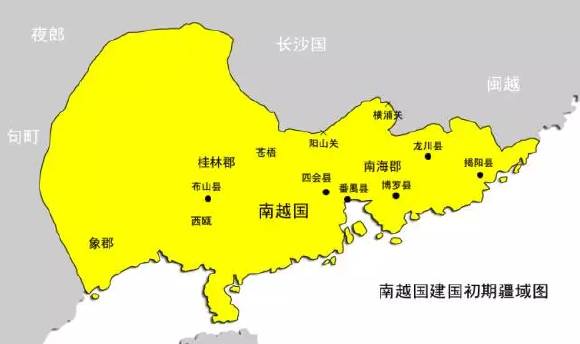
\includegraphics[width=\textwidth]{images/image-8}
	\caption{南越国初期疆域图}
\end{figure}

赵佗是很现实的人。吕后很快就死了,长沙王是顶不住南越的。后面就是文帝了,文帝又派使者跟南越说,我们不要打了,只要你们给我们一个面子,就不打了。然后赵佗说,好好好,我称臣,以后我又是王,我不是皇帝了。但是我们可以看到,这个跟后来越南历史的情况如出一辙。越南对中国就一直是这样的:我对中国说我是王,你是皇上;但是他关起门来就说我是大越国皇帝。赵佗也是这样,他关上门还叫自己是皇帝。

其实赵佗是哪里人呢?是河北人。但是他到了南越这个地方以后,他是遵从越俗的:文身断发椎髻;饮食,我们从南越王的墓里面能看到他吃的东西也都是南方的东西,鱼蛇鳖之类的。赵佗在国内的称号叫做“蛮夷大长老”,他给汉朝写信也管自己叫蛮夷大长老,等于说他已经把自己当成一个越人了。赵佗最后活得非常久,他统治南越统治了七十多年。公元前137年他死的时候已经是汉武帝的时代了,他出生在战国时代,活到汉武帝的时代,活了103岁,我们可以看到有德性的人非常有好报。


\begin{figure}
	\centering
	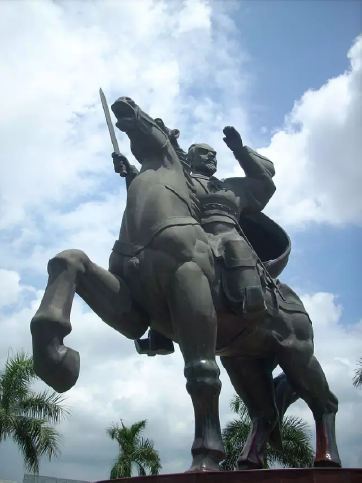
\includegraphics[width=\textwidth]{images/image-9}
	\caption{河源县赵武帝(赵佗)像}
\end{figure}

他死了,他的儿子其实已经都死了,活不过他。登基的就是他的孙子,叫赵眜(南越文帝)。赵眜在位期间为前137年~前122年,在位一共16年。今天广州有一个南越王墓就是他的墓,我们就能看到那个墓里的很多东西,非常精美,还有玉衣,他的遗体穿着玉做的衣。赵眜统治时期发生了一件事情,就是东边福建的闽越国攻打南越。赵眜不敢自己发兵,他想,如果我发兵,那汉朝问罪下来怎么办呢。于是他向汉武帝求救。然后汉朝就说,你很乖,然后派人去打闽越。但是汉朝军队走到一半,闽越内部发生政变,原来的国王被杀掉了,结果战争没有打起来。就是这样一件事情。

这件事情之后,赵眜怕汉朝,于是他就把他的太子赵婴齐送到了长安,入朝朝见汉武帝。赵婴齐到了长安之后,就娶了一个当地的女人叫樛氏,是一个河北邯郸的女人,然后生了一个儿子叫赵兴。赵眜死了以后他就回来登基,他带着他在北方娶的老婆还有在北方生的孩子回来登基。这个人就是南越明王(注:赵婴齐即位之后,废去了赵佗、赵眜在位时所称的帝号,在国中改称“国王”,将先帝的玉玺藏于国库中不再使用。),第三代君主。南越明王,其实没什么太可说的,他干了七年(BC122~BC115)。七年之后就是南越哀王,赵兴。

\begin{figure}
	\centering
	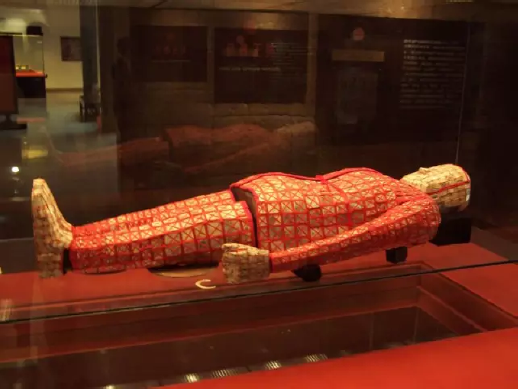
\includegraphics[width=\textwidth]{images/image-10}
	\caption{南越文王墓出土的丝缕玉衣}
\end{figure}

\begin{figure}
	\centering
	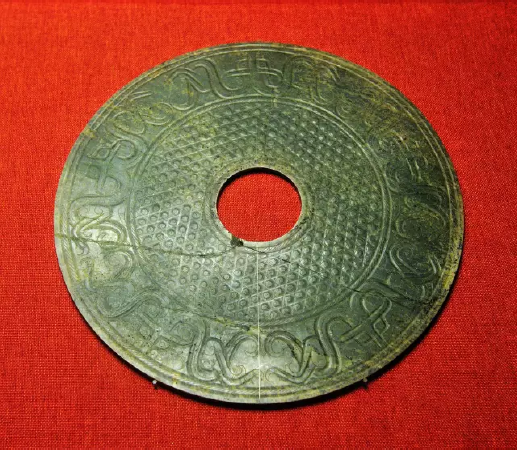
\includegraphics[width=\textwidth]{images/image-12}
	\caption{玉衣上的谷纹夔龙纹玉壁}
\end{figure}

赵兴登基的时候年纪很小,于是桂枝式王朝一种常见的现象就出现了,就是太后专政。而这个太后是哪里人呢?是河北人。所以这个太后对南越是没有感情的。这个是公元前113年的事情:等于说被一个河北人给掌握了政权,被绑架了,这个时候武帝很高兴,好~你们赶紧再来入朝,然后他派了一个人叫安国少季。安国少季是个什么人呢?他是太后以前在北方的情夫,是姘头。安国少季来了,太后一见如故,很饥渴,两个人就搞上了。搞上了之后,安国少季跟太后说你们要入朝。太后说,好好好,一定入朝,归附大汉,然后说,以后三年朝见天子一次。哀王其实也没什么好说的,哀王说,好好好,母后说的是。基本上这个投降卖国的条约已经要签成了。

这个时候南越的丞相吕嘉不干了。我们知道从赵佗时代以来,南越一直奉行的是越化政策,它的百官有非常多的越人。吕嘉也是一个越人,他怎么能容忍他的祖国被北方来的、完全不融入当地的这种太后、这种反动的势力所控制呢?于是在公元前112年,吕嘉就发动越人起兵,杀掉了太后、哀王还有安国少季,然后又击败了来进攻的汉军,又另立了一个小皇帝叫赵建德。吕嘉起兵的时候,号召的檄文是非常的激动人心的,我们看一下:

\begin{quote}
王年少。太后中国人也,又与使者乱,专欲内属。尽持先王宝器入献天子以自媚,多从人行,至长安,虏卖以为僮仆,取自脱一时之利,无顾赵氏社稷为万世虑计之意!
\end{quote}

太后不是我们的人,又要“与使者乱,专欲内属”,自由的南越人是绝对不能答应你们这样的。你们还把先王的宝器都送给汉朝了,要“自媚”。你们带走很多随从的人跑到长安去,把他们卖给汉人,然后再从人口买卖当中取利。你们根本就不顾先王的社稷。


\begin{figure}
	\centering
	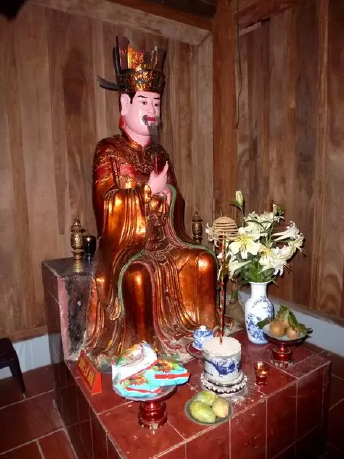
\includegraphics[width=\textwidth]{images/image-13}
	\caption{越南河内市怀德县的吕嘉像}
\end{figure}

这个很有意思。赵氏其实是哪里人?也是河北人。但是在这里面,他们认为赵氏是河北人么?不认为。其实这个也是后来南粤史的一个特点:就是说你到这个地方之后,你必须要认同这个地方;如果你不认同的话,那你就不是自己人。

这个是一个非常有战斗性的檄文。吕嘉丞相很伟大。但是汉武帝就生气了。我们知道,阿姨说过他是文明的收割者,他其实比秦始皇还要残暴。于是汉武帝就派了伏波将军路博德,带了十万人去攻打南越。南越撑不住的。吕嘉丞相带着赵建德坚守番禺,就是广州城。汉军纵火焚城,打了进去。最后赵建德被俘,吕嘉丞相被抓以后就殉国了,被杀害了。南越就亡国了(BC111)。

这样,南粤历史从公元前203年到公元前111年,大概是九十几年的一段自立历史,这是南粤历史上的第一个自立的王朝。汉朝打下这里之后,我们看到它设了九个郡(儋耳、珠崖、南海、苍梧、九真、郁林、日南、合浦、交趾),比秦设的三个郡要更多,这是什么意思?更有利于统治。因为郡县,我们可以把它理解成帝国的神经节点。这些地方,“儋耳”跟“珠崖”就是海南,“交趾”、“日南”和“九真”是今天的越南,“南海”就是广州,“苍梧”就是桂林,“郁林”在桂林附近,“合浦”是今天雷州半岛。等于用九个郡,用九个这种大的殖民点,进行了更深一步的管制。于是南粤开始了第二次北属。


\section{第二次北属}

我们可能以前在高中学过,说汉武帝设了十三州(BC106),他不放心地方的官员,不放心郡县,于是他又把天下划为十三州,每个州派一个刺史,这个刺史每年的俸禄是六百石,地方的郡太守是两千石,用刺史这种更低级的官员,去管理相对在地方上有割据势力的官员。这是费拉帝国的一贯心法。十三州的其他州都叫×州×州×州,只有南粤不叫州,直接叫交趾,包括今天的广西东部、广东,还有越南北部,这个地方是不叫州的。汉朝觉得这个地方是不一样的,其他的地方都是在它的地盘上,这个地方就是一个殖民地,不是华夏的州。因为这个地方相对来讲,地理上比较隔绝,等到西汉完蛋之后,当地的地方官就又闭关自守了,但是也没有独立,就是说谁是老大我向谁称臣。这个地方没有遭到两汉之际的大洪水的波及。

到了东汉初,它又归附了东汉(AD29)。在东汉有一件比较大的事情,就是在交趾郡,在越南境内出现了两个女子,叫征侧跟征贰。征侧的丈夫被汉朝的官吏给杀了,于是她们就率领越人进行了大规模的起义,把交趾、九真、日南三个郡全部都打了下来,然后把当地的汉朝官员杀掉。最后汉朝又是派兵镇压,派出的将领是伏波将军马援,他是东汉的一个开国功臣。马援一下去就把起义镇压了下去,二征自杀。这个是汉朝治下的几件大事。



\begin{figure}
	\centering
	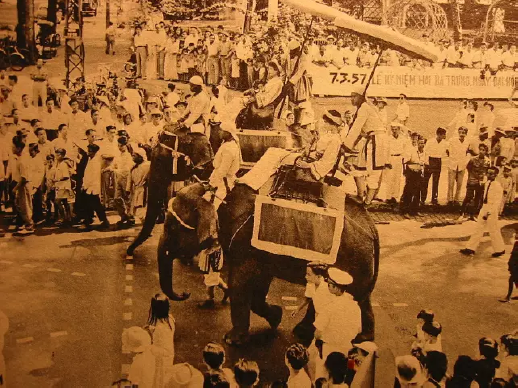
\includegraphics[width=\textwidth]{images/image-14}
	\caption{越南举行的二征起义记念活动}
\end{figure}

再后面就是三国了,桂枝本部是三国,离南粤最近的就是孙吴,但是孙吴一开始还不是太强。我们知道,184年是黄巾之乱,汉末大洪水爆发。当时天下大乱之后,又有一个人站了出来,他像赵佗一样站了出来,这个人叫做士燮。士燮不是北方人,他就是本地人,他是苍梧人,他在越南北部的交趾当太守(187年,士燮被汉朝任命为交趾太守)。我们可以看到当时的越南跟南粤其实是一体的。士燮是一个大土豪,他又当了地方官,虽然他其实是广西人,他在越南当官,但这些地方当时是一体的,等于就是在本省当官,我们可以这样理解。他就把他家族、乡党全部聚集起来自卫,然后把他的兄弟全部都安插到各个郡,九个郡有七个郡都被他的兄弟还有亲戚给控制了。士氏就成了当地的实际的掌权者。但是不像赵佗那样,他没有自立。

\begin{figure}
	\centering
	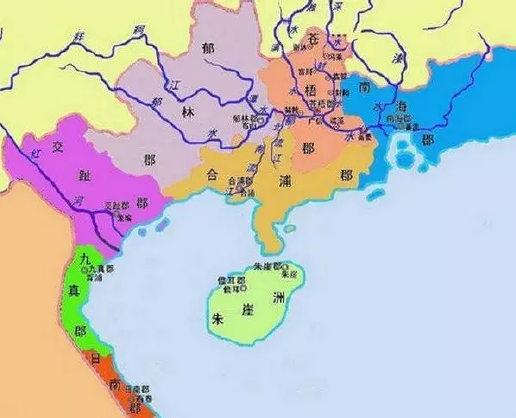
\includegraphics[width=\textwidth]{images/image-15}
	\caption{岭南九郡}
\end{figure}

孙吴慢慢强大了,他在公元208年打赢了赤壁之战,于是他要把目标放向南方。因为当时孙吴面对着一个很大的问题,我们知道,孙吴的阶级基础是江东的豪族,孙吴的皇帝想打仗的话,他相对不太容易直接控制那些豪族的兵,那些豪族都是世袭的部曲,等于是一种封建制度。那么他的兵源从哪里来呢?他就要打外面的百越人,从百越人里抓俘虏。我们课本上有一个很扯淡的话,说什么孙权派卫温、诸葛直到台湾,最早跟台湾友好交流。其实去干嘛了呢?抓了几千个人,就干这种事情,汲取(《三国志·吴志·吴主传》:“(黄龙)二年……遣将军卫温、诸葛直将甲士万人浮海求夷洲及亶洲。亶洲在海中,长老传言秦始皇帝遣方士徐福将童男童女数千人入海,求蓬莱神山及仙药,止此洲不还。世相承有数万家,其上人民时有至会稽货布,会稽东县人海行,亦有遭风流移至亶洲者。所在绝远,卒不可得至,但得数千人还。”)。接着他就把目光瞄准了南粤,这个地方抓人太好抓了。


\begin{figure}
	\centering
	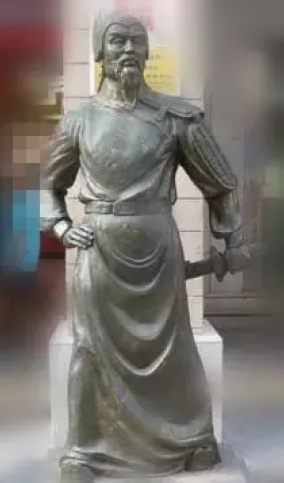
\includegraphics[width=\textwidth]{images/image-16}
	\caption{士燮}
\end{figure}

于是孙权就派了一个人叫步骘,大家可能玩过三国志会看到这个人,这个人在三国志里面能力不是太强。他是文官,让他当交州刺史(210~220)。步骘新造了一个比较大的广州城。但是步骘,我们可以看到,他也很难说打到基层去,因为他是一个刺史,而地方官都是士燮的家人。

然后孙权在220年又派了另外一个人叫吕岱,看过《三国演义》的都应该见过这个人,派这个人替代步骘做交州刺史。226年,士燮就死了,去世了。其实他也是一个割据自保的人,我们看到大洪水基本上跟南粤没关系。他也是很有德性,得到了很好的结局,90岁,跟赵佗差不多高寿。士燮就相当于南粤的一个守卫者,他一死,这个吕岱就敢下手了。于是吕岱就把交州给分成了两块:一块是交趾、九真和日南,这个地方叫交州;北边几个郡叫做广州,他自己当了广州刺史。然后派戴良为交州刺史,要把自己的人安插到北边的这几个郡来,那么这样的话他其实等于是在分割士氏的势力。士燮的儿子叫士徽,他非常清楚这一点,就举兵阻拒戴良入境。于是吕岱就去打他们。

\begin{figure}
	\centering
	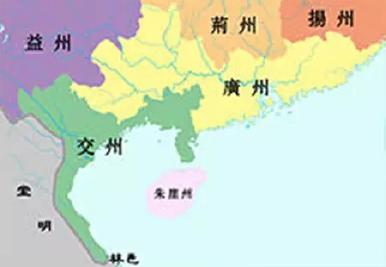
\includegraphics[width=\textwidth]{images/image-17}
	\caption{264年,孙休析交州北部置广州}
\end{figure}


打了之后,士徽觉得打不过,打不过怎么办呢?吕岱和士徽的堂弟士匡有交情,这个时候就派士匡跟他说,你可以投降,你把你的部众交给我,我绝对不会杀你。但士氏投降之后,吕岱就把士氏主要成员都杀了。我们后面还能看到,何真等于是这个故事的翻版,你如果死扛到底可能就没这些事情了。只有那个叛徒士匡没有被杀,给他养到北方去了,也不知道他面对自己家人被杀的情形,是什么心情。士氏被消灭了之后,孙吴又把广州跟交州合在一起了。这样的话,孙吴就把岭南又一次自立的势力给彻底的铲除掉了。

接着,南粤就变成了吴国跟魏国争夺的战场。我们可能觉得奇怪,魏在北方,他怎么过来呢?因为魏国跟吴在正面对峙的同时,他也想从后面给吴背后捅一刀。而且我们知道,孙吴打这些地方本来是为了什么呢?为了抓人,而且这个地方海外贸易发达,有很多外国的珍宝。于是孙吴就各种抓人,强征珠宝,整得这个地方苦不堪言。最后这个地方又有一个小土豪,他是一个小的吏员,郡吏,叫吕兴,他在公元263年以交趾三郡——交趾、九真、日南一起造反,投降了魏国。这样的话,交州和广州等于又分开了(264):原来吕岱划的广州那一块,就是今天的广东广西,这个地方还忠于吴国;而越南已经忠于魏国了。交州、广州在这之后就永远得分开了。

\begin{figure}
	\centering
	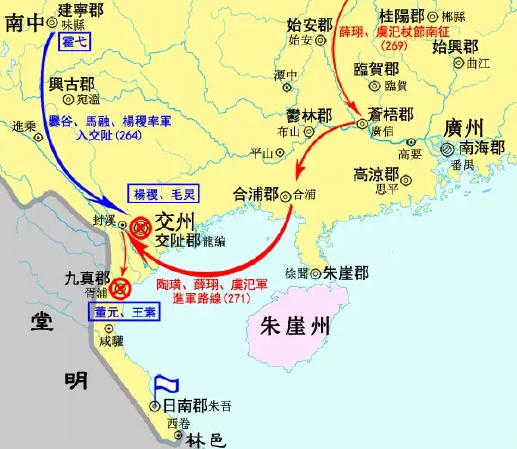
\includegraphics[width=\textwidth]{images/image-18}
	\caption{吴魏交趾之战}
\end{figure}


接着,交州、广州之间,魏国跟吴国的势力以这个地方为战场打了八年(263~271)的战争,这个地方已经再也没有像士氏那样的土豪去保证它的一方安宁了。这个地方等于说第一次沦为帝国大洪水的牺牲品。后来魏国在265年变成了晋,那就是晋跟吴在打,打了八年。最后吴在271年终于把交州给打了下来。这个地方一片残破。吴在南粤搞的这些暴政非常不得人心,打了这么多年仗,疯狂的汲取。于是在吴灭亡的前一年——当时吴的皇帝是孙皓,那个人很残暴的,喜欢剥人脸皮——广州有一个人叫郭马,他就带着广州人起义,把这个城占了(279)。然后孙皓就派一支一万七千人的军队去镇压。然而第二年吴就灭亡了(280),然后岭南就归于晋朝。至于郭马本人的下落,史书未载,很可能最后被西晋残酷镇压了下去。这个就是帝国大洪水第一次波及到岭南。

再后面就是东晋。其实我们知道,西晋没玩儿几年,他自己就内战起来了,接着五胡就来了。五胡一来,很多氏族就南下,有一小部分氏族就到了南粤。这些人也是以殖民者的心态来到这个地方的,他不会对这个地方的粤人有太多的爱,很少。又有一场大洪水很快又波及到了这里。我们知道东晋末年有一个孙恩卢循之乱(孙恩之乱399~402;卢循之乱403~411),孙恩卢循他们是信道教的五斗米道,其实就是跟日后的白莲教、义和团很相似。他们是从吴越这个地方出发,然后一路往南抢,抢到岭南跟越南,然后再北上,最后沿着赣江、长江把江西、湖南、湖北抢了一遍,就这样四处流窜、转圈圈,转了十几年,最后在越南被消灭的。他们当然也进了广州了,打下了广州,曾经在404年的时候打下了广州,放了一把火,烧死了一万多人,然后在这个地方盘踞了六年之久(404年11月~410年11月),最后在411年才被干掉。当时这个时候东晋很快就要完了(420)。后面就是刘宋刘裕,已经到南朝了。这个是第二次被大洪水波及。

\begin{figure}
	\centering
	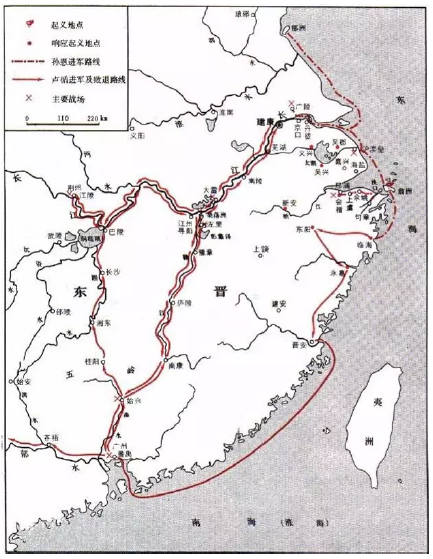
\includegraphics[width=\textwidth]{images/image-19}
	\caption{孙恩卢循行军路线}
\end{figure}

南朝治下,我们看到南粤基本上已经没有赵佗跟士燮这样的土豪了,那么它就沦为帝国权力斗争的一个舞台,没有人去自保了。南朝宋就有两个帝国内部官僚在南粤掀起叛乱,一个叫萧简(453),一个叫袁昙远(466)。袁昙远叛乱的时候,又大掠了一把广州。大家想想,为什么喜欢去掠广州?有钱嘛。而且你没法自保了,不掠你掠谁,你已经丧失了自保的能力了,你就是一个肉猪。

这种情况直到南梁的末期才有所改变。我们知道,梁朝的梁武帝萧衍,在他的治下南朝享受了45年的和平,但是萧衍的晚年发生了一个侯景之乱。侯景是北方北齐的一个将领,他是一个胡族的将领,然后他跑到南方之后,就掀起了叛乱,他想篡位,夺取大权。他的部队沿着长江一路从湖北这个地方往东打,包围南京一百多天,最后梁武帝就是被饿死的。那么这个时候,整个长江流域又发生了一次大洪水。

但是这个时候终于出现了一个有土豪德性的人,这个人就是陈武帝陈霸先。陈霸先就是南朝最后一个朝代——宋齐梁陈那个陈的开国君主,陈武帝。我们知道,宋齐梁的君主,他们是北方人,他们都是北方南逃过来的氏族。但是陈霸先不是,陈霸先是吴越人,他是本地人,所以说他对南方是有一种爱的。当时他正在岭南当官,当西江督护,管西江沿线的这些军事。他听说北方乱了,然后他就召集了南粤的一批义兵。他在南粤是比较能服众的,他跟本地人关系不错,然后北伐,南粤兵一直到南京,最后把侯景打败(552)。接着又以这些兵为基干,打败了南侵的北齐。这个等于是南粤武功的一个复兴吧,靠着一个有土豪德性的人。最后陈霸先就把这个梁给篡位了,建了南朝第一个也是最后一个本土王朝,陈朝(557)。

\begin{figure}
	\centering
	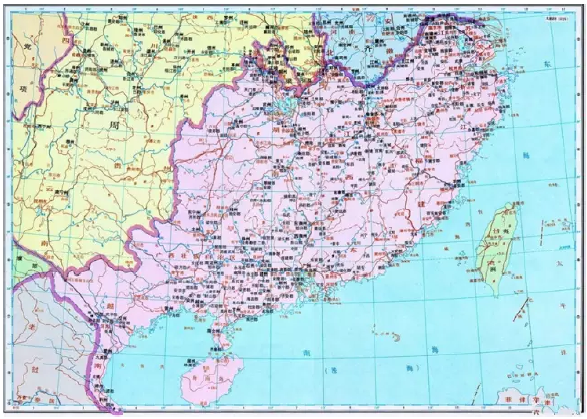
\includegraphics[width=\textwidth]{images/image-20}
	\caption{南朝陈疆域图}
\end{figure}

陈武帝当了几年皇帝就死了,陈朝接着也就维持不下去了,也要不行了。因为我们知道,其实陈武帝毕竟不是南粤本土的土豪,他没有留在南粤,陈朝最后也变成一个帝国。广州就再次变成陈朝战乱的牺牲品。有一个人叫欧阳纥,他也是一个广州地方官,他就造反(569),最后官军打进来,又大抢了一把。

\section{冯冼政权}

直到陈朝末年,终于又出现了一批自立的人。这个就是第二次自立。出现了两个人,一个叫冯宝,一个叫冼夫人。当时我们看到的南粤,汉人会住在沿江分布的殖民点。而粤北、粤东、粤西这些广大的山区,都不是汉人。当时粤西的蛮族,最大的两支,一支叫僚人,一支叫俚人。俚人的核心区域是在粤西的丘陵地带中,今天的高州,也就是茂名以北那块地方。当时俚人有一个很大的豪族,叫冼氏。我们可以看到他们采取的是汉人的姓氏,所以说他们其实跟汉人是有很多交流的,他们吸收了汉人的命名方式。俚人大族冼氏,当时说有十余万家在那个地方,是个大部落,一家假如说五个人,就有五、六十万人,很大规模的一个团体。他们的大首领是个女的,就是冼夫人冼珍。

\begin{figure}
	\centering
	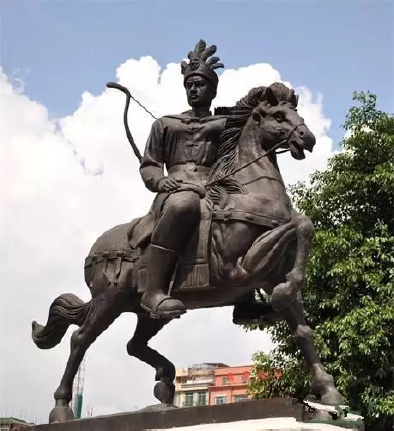
\includegraphics[width=\textwidth]{images/image-22}
	\caption{冼夫人像}
\end{figure}

南朝末,我们刚才看到欧阳纥之乱,等于说广州已经乱了。粤西的高凉太守冯宝,他也是陈朝的官员,但是他很懂得跟当地的势力合作,他就娶了冼夫人,两个人联姻,然后这个冯氏也变得粤化了。他们一起联手帮助陈霸先,不但是出兵帮陈霸先打侯景,后来还帮陈霸先把欧阳纥给讨平了。那么在这样的情况下,其实我们也可以说,陈霸先的德性最后培养出了这样一个集团,冯冼集团,于是又有了一个自立的可能。而这些自立的人,我们可以看到,之前的那个士燮,他们是住在城里的,他们是很汉化的一个家族;而这个是一个很蛮族化的家族。那么这个是一个什么现象呢?那些汉人这个时候已经不太可能说再去恢复一个自立的政权了,这就是蛮族在输入秩序。于是冯冼集团这个部落在军事上,在他们消灭了欧阳纥之后,已经控制了南粤。

最后,公元589年的2月,隋朝南下,把陈朝灭了。当时冯宝已经死了,南粤地方又自保,奉冼夫人为圣母,给她一个称号叫圣母。于是南粤出现了第二个自立的政权。这个政权只维持了九个月,到11月就不自立了,投降了隋朝。我们看冼夫人这种行为:投降了隋朝,接着又把另一个反隋的、也是俚人的大帅王仲宣给杀掉了(590),我们看到好像她是一个粤奸。但我觉得她的行为更多的是像跟隋朝做了一笔政治交易,就是我在政治上臣服于你,但是你要给我自治权。这个东西在隋朝看来,是这个蛮夷归化我们了,蛮夷对我们向化了;但是如果我们能看到冼夫人一方的记载的话(当然我们根本看不到俚人的文字了),可能他们就是觉得,我们骗了这些傻乎乎的北佬,我们向他们投降,然后我们保留了自己的自治权。

冼氏在南粤可以开幕府,这个幕府不是日本的那个幕府,就是说可以自己建官,设官职,派官僚,还可以设官署,在各地控制地方官,还有军权。等到冼夫人去世的时候,602年,这个时候还有两年就到隋炀帝了。她的两个孙子,冯暄跟冯盎,又继承了她的事业。其实冼夫人也活了很久,活了九十岁。南粤历史有一个现象,这些德性很好的人都活了很久。

\begin{figure}
	\centering
	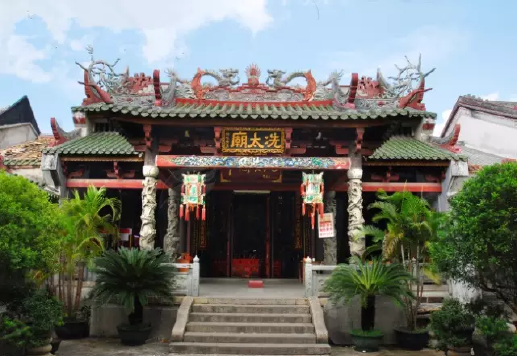
\includegraphics[width=\textwidth]{images/image-23}
	\caption{冼太庙}
\end{figure}

除此之外,当时在合浦,就是雷州这个地方,还有一个大豪族叫宁氏,他们是汉人,但是他们跟冼氏是结成了同盟,他们也保住自己这一方,保境安民。等于说冯冼集团和宁氏在奉隋朝为君主的前提下,实际上在这个地方独立了。在隋朝是这样的一个局面。我就说它是无独立之名有独立之实。

后来就是隋末大洪水了,天下又是一片战乱。南方出现了一个人叫萧铣,他是南梁的后代,他想恢复梁朝;还有一个姓林的人(林士弘),他建了一个楚国。他们在北方争霸。北方两大强权争霸,宁氏跟冯氏很有意思,他们各选了一个老大,一个奉梁的年号,一个奉楚的年号,然后两边打仗。他们真的是为外敌来卖命么?恐怕也不是。这个只是南粤内部的一个事务,他们只是换一个名义上的效忠对象,等于还是自己内部的一个事务,跟北方没什么关系。

最后我们看到,后来他们两家找的老大都完了,唐朝出现在北方。在公元622年,他们就归附了唐朝。631年,冯盎就去朝见了唐太宗,又得到了唐太宗对他们自治的认可。所以说从陈末到现在为止,已经差不多过去了有五、六十年了,这个政权已经维持这么久了,他们顶着这个帝国的帽子,以蛮族为基础,已经维持这么久了。但是最后,这个政权还是走向了一个悲剧的结局,这与武则天有关。

\begin{figure}
	\centering
	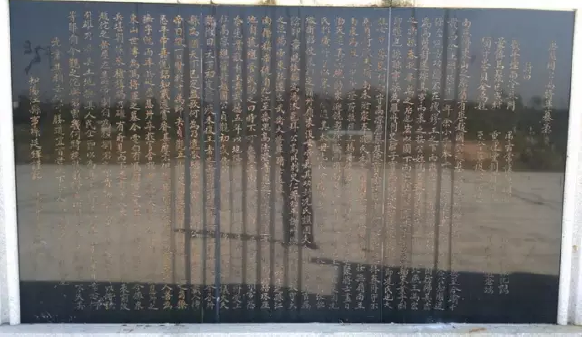
\includegraphics[width=\textwidth]{images/image-24}
	\caption{唐越国公冯将军(冯盎)墓表}
\end{figure}

武周革命其实是一场什么样的革命?隋唐的建立者是关陇集团,他们是很鲜卑化的。最早隋唐的蛮族是怎么进来的?是北魏先汉化了,但是北魏在北方留了一帮穷兄弟,最后他们不满中原的汉化,于是他们打了进来,把北魏公卿都杀光光。这个叫六镇之乱(524)。后来有一部分人到了关中,形成了一个西魏政权;西魏后来变成了北周,北周灭掉了关东的北齐,就统一了华北;最后北周又被杨氏篡位,变成了隋。其实隋唐的皇室都是这个集团里面的,他们就是鲜卑蛮族的一个集团,又称为关陇集团。其实唐初的政权基本上就是这个集团所把持的。

但是武则天不一样,她不是这个集团里面的人,她是汉人。所以她上台了之后,她就要打击关陇集团,靠科举上来的文士去分割关陇集团的势力。她就是一个没有什么政治德性的人,她觉得你在南方有一个割据的势力,肯定要把你给铲平掉,不能容忍你。反而是关陇集团可以容忍他们的存在,因为关陇集团可能觉得他们跟我们其实是同类,因为我们都有蛮族背景。

武则天上台的第三年(693),首先说岭南的流人——就是当时帝国有很多人会被流放到那里,说他们要谋反,一口气杀了三千多人。接着又说南方的僚族要谋反,俚人要跟他们勾结。在冯氏里面挑了三十六家比较厉害的,把他们全杀了(694)。但是冯氏还能忍,居然也没有造反,也没有死磕到底,等于还有幻想。

又过了三年,武周就直接说冯冼这两家是叛逆,直接派兵南征,攻破了高州(697)。这个是非常壮烈的一幕,冯氏的男丁为了保卫高州城一个接一个地战死,跟武周军队战斗到了最后一刻,许多男丁都光荣的战死,这是非常壮烈的一幕。接着,武周的军队打进高州城之后,把他们的家产全部都没收,把隋唐帝国赐给他们的这些东西,官服什么的全部都毁掉。我们看,冯宝跟冼夫人的这个势力维持了多少年?有一百多年了。从陈一直到接近唐中期,就以这个悲壮的战争为结尾结束。于是岭南又一次落入了帝国的控制当中。

\section{第三次北属}

唐朝治下的岭南,我们知道唐太宗把天下分为十道(627),其实跟刺史差不多,有点像后来的省。五岭以南为岭南道。后来到了862年,又把这个岭南道分割成两部分,岭南西道和岭南东道,岭南东道就是今天的广东。697年,冯氏跟冼氏被帝国消灭了。705年,唐朝发生了唐中宗复辟,把武则天给赶下台了,但是其实这并没有造成关陇集团的复辟,对各共同体的打压还是延续了武则天的路线。武则天已经干掉了冯氏跟冼氏,这时唐中宗就把剩下的宁氏,就是那个汉人的豪族,说宁氏也是叛逆,把他们给干掉了(706)。这样的话,等于说所有的这种自治力量又一次被帝国给摧毁了。

\begin{figure}
	\centering
	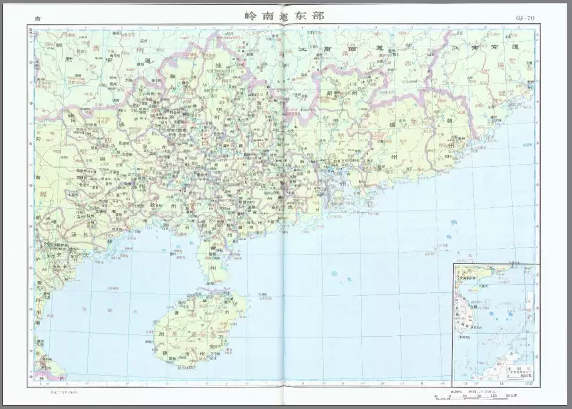
\includegraphics[width=\textwidth]{images/image-25}
	\caption{岭南道东部}
\end{figure}

当地还有一些豪族,他们是跟着冯氏、冼氏和宁氏的,他们肯定不能甘愿做帝国的奴隶,我们已经自治了一百多年了,你们怎么能这样就消灭我们天赋的权利呢?于是在公元728年,这个时候是唐玄宗的时候了,所谓的开元盛世——我们知道这种盛世其实就意味着帝国机器的空前强大和虚假的繁荣——两个大豪族,一个叫陈行范,一个叫冯璘,他们起兵,以广州为中心,占据了四十多个城,然后说我们要恢复南越,称南越王。然后唐玄宗又派大军去打他们,这一次一口气在广州杀了六万多人,把这个起义给残酷地镇压了下去。这样,岭南就彻底地又一次变成了降虏了。从陈朝的末年到这个时候,大概已经有一百五十年了。

接着,我们知道,唐朝有一个很重要的赋役改革叫两税法(780),就是每个人都要夏天交夏税,秋天交秋粮,夏税秋粮,由国家统一核算。实行这种税法,你就必须要做到对你人口的控制,你必须得知道有多少人,我才能计算我能收上来多少税。于是就对俚人进行大规模的编户齐民,向他们征税。这些人已经没法反抗了,因为反抗的人都已经遭到屠杀。于是这些俚人就汉化了,我们今天看不到俚人了,我们只能发现粤西的很多人长得确实很不“汉”,但是今天他们已经成为了所谓的汉族。我们知道汉族往往是一个什么含义呢?就是降虏,就像那些埃及人一样。

唐朝的最后一幕就是黄巢大洪水。黄巢,我们知道,他是到处流窜的。公元879年他流窜到了广州。打下广州之后又来了一次屠城,一口气杀了十几万蕃商,因为这些人最有钱。对于这种级别的流寇,其实已经无力抵御了,没有豪族了。等于说帝国大洪水一来,它的大洪水也就一起跟着来了。

\begin{quoted}
某听众:安史之乱的时候这边是什么情况?

执经生:那倒没什么事。安史之乱就在江淮那边,南不过江淮,所以安史之乱时这边反而没什么事。
\end{quoted}

\section{南粤史前半期之南粤社会}

以上就是南粤史的前半期。我们看到前半期的南粤史有一个特点:这个地方汉化的程度不深,直到唐朝才有点汉化的样子。对于帝国来说,这个地方相当于一个肉猪。帝国最怕的是这个地方的人不归他管,怕这个地方的人造反。如果有造反的话,比如说像赵佗、士燮还有冯冼,都要残酷屠杀你,不能让你有活路。我们看到,南粤历史前半期的几个机会窗口,最后都被帝国堵住了。所以说这个地方对帝国来说就是一个殖民地,而且是这种西班牙帝国在南美洲的殖民地,是这个含义。我们可以把帝国就理解成那种穷凶极恶的西班牙殖民者,而当地的粤人就是印第安人。他们其实很有武德,但他们一次次的反抗都被帝国一次次的大屠杀。

那么我们就看一看这段时间南粤的社会风貌。首先看广州,当时的广州是什么样?不是今天的广州这个样,它是很异域风情的,它不像一个所谓中国的地盘。因为从汉朝以来,帝国是一直跟印度和中东、北非都是有海上贸易的,广州就是这条所谓海上丝绸之路的最东端,所以这个地方肯定是有很多外国人的。我们今天很多人好像觉得广东有很多黑人就是很大件事一样,其实这一直是一个传统。历史上,广州一个特点就是“华夷杂处”。西晋初的时候,罗马的商人都很可能到过南粤的。

\begin{figure}
	\centering
	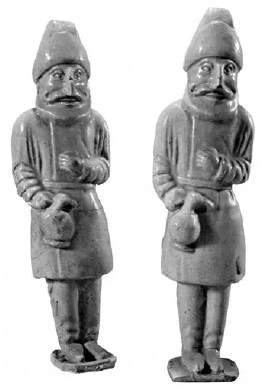
\includegraphics[width=\textwidth]{images/image-27}
	\caption{广州出土的唐代阿拉伯人佣}
\end{figure}

唐代的广州,当时的人就有一句话:“蕃獠与华人错居,相婚嫁,多占田营地舍。”“蕃”就是外国人,“獠”就是土著僚人,与汉人杂处,互相结婚,这些人还有很多财产。“多占田营地舍”,这表示怎么样?表示在这个地方安居下来了。广州人想出去也很方便,他可以去去中亚、去印度,坐船就过去了,因为有一条航线。唐代在广州这个地方设了一个机构叫市舶司,就是海关,就是一个汲取的机构,把这个地方当作捞钱的地方。

当时广州的整个宗教氛围,在后世的理学儒家士大夫看来是很可怕的,对他们来说广州到处都是一些异端的思想。佛寺跟清真寺非常的多。比较大的几个佛寺,这几个寺今天都在:光孝寺、华林寺和六榕寺。光孝寺是印度人建的(401),有一件比较大的事,就是六祖慧能是在光孝寺剃度的(676)。光孝寺在刚刚建的时候不像今天都是一些中国的僧人,这个地方很大程度上是一个给印度人歇脚的地方。还有华林寺(526),华林寺是禅宗的始祖达摩刚刚入华的时候居停的地方。还有一个六榕寺(537),这个是南梁自己建的,这个是比较华夏风格的一个寺,印度风格不明显。当时的广州,是居住着不少印度人的。还有一个极大的清真寺就叫怀圣寺(627)。我们看到阿拉伯人也就是622年创立了伊斯兰教,没几年他们就来到南粤,来了就建了清真寺。这个寺今天也在,是一个很清真的地方。

\begin{figure}
	\centering
	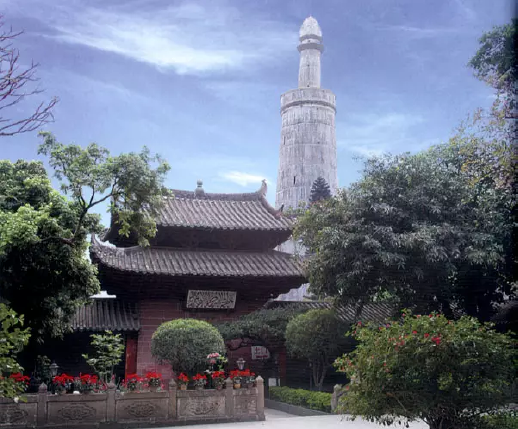
\includegraphics[width=\textwidth]{images/image-28}
	\caption{圣光寺}
\end{figure}

据说唐代的广州有十几万外国人。当时的广州也不到一百万人,也就是几十万人口,加之城里还住着许多土著,估计城内一半左右的人都不是汉人。它就是一个光怪陆离的世界,你在那里能看到来自世界各地的人,你能看到印度人,能看到阿拉伯人,能看到黑人,能看到波斯人,甚至能看到来自西欧的人,能看到汉人,又能看到各种岭南的土著。香港都不是这种感觉,说真的,香港还是一个以粤人为主的社会。今天或许已经没有这样的城市了。

这里有一段材料,大家看看当时的世人是怎么写南粤的风俗的:“家有人病,先杀鸡鹅等以祀之,将为修福。若不差,即刺杀猪狗以祈之。不差,即次杀太牢以祷之。更不差即是命也,不复更祈。死则打鼓鸣钟于堂。比至葬讫初死,但走大叫而哭。”(《太平广记》)

当时,粤人在家人生病时,会杀掉大量的牲畜,“不差”就是没用,我先杀鸡鹅,没用,那我就杀猪狗,没用,我就杀太牢,我就杀牛羊猪,没用,那好吧,等死。在汉人看来,这些人就是难以理解的一些神经病。这是宋代人记的唐代人的话,《太平广记》是宋初的东西。而且这些人没有任何儒家的礼仪,死的时候,就要在堂上、在停灵的地方敲锣打鼓,这些人一边跑一边叫。我们可以看出来,唐代人跟后来的宋儒不一样,他们想改变这些人么?其实也不想,就觉得这些人神经病而已。这些汉人觉得,自己对于南粤而言是外人,与粤人不是一种人,完全就是两个世界的人,南粤就是一块殖民地。就像西班牙人到了南美洲,就觉得这些印第安人真奇怪,就是这种感觉。

还有一个故事,这个是唐代人写的:山魈者,岭南所在有之。独足反踵,手足三肢,其牝好傅脂粉,于大树空中作窠,有木屏风、帐幔,食物甚备,南人山行者多持黄脂、铅粉及钱等以自随,遇雄者谓之「山丈」,遇雌者谓之「山姑」,必求脂粉,与者能相护(《广异录》)

“山魈”的生活是很奇怪的,住在窠上,就是干阑,汉人在城里住的是房子,这些人住的是干阑。其实这些就是人,土著初民就是这些人。他们为什么会喜欢黄脂、铅粉这些东西?他们可以想象,西方人刚到非洲,非洲人最喜欢的是什么?玻璃球。就是些奇奇怪怪的东西,好看,他们没见过,你看这个脂粉多有意思,他们就喜欢这个东西。我们就可以这么理解。

再后面:其岁中每与人营田,人出田及种畲耕地种植,并是山魈,谷熟则来唤人平分之,性质直,与人分,不取其多,人亦不敢取多,取多者,遇天疫病。(《广异录》)

我们可以看到这句话:“人出田及种畲耕地种植,并是山魈”,是谁来种地的?人跟“山魈”,人是出田的,“山魈”出力。“山魈”在经济上是受制于人的。但是人不能像奴隶一样对待他们,因为他们“性质直”,你“不敢取多”。取多者,所谓的疫病,我估计其实就是被他们干掉了,你不敢多取。其实这些“山魈”是什么人呢?就是粤人。这就是汉人写的东西,他觉得他们都是怪兽,不能理解他们。但粤人又是很有德性的人,汉人不能把他们逼得太急,但他们经济上又受制于汉人,就是这样的一个情况。

还有一个就是各种“异物”,就是在北方人看来没见过的,荔枝、椰子、犀角、玳瑁(乌龟壳)、珠宝、瘴厉。因为北方人说来这里太热了,受不了湿热就挂了,得了一个什么病就挂了,对于北方人,南粤这个地方就是外国,中原都不产这些怪怪的东西。

当时本地也是有粤人士大夫的,汉代就有一个最有名的,治《春秋》的,他的《春秋》学非常厉害,他叫陈元,是苍梧人,苍梧就是在西江上。唐代很有名的张九龄,大家都知道,曲江人,曲江在韶关,韶关在北江边上。所以说士大夫传统上都住在哪里?都住在沿江分布的城市,这些人都是殖民者的后代。

\begin{figure}
	\centering
	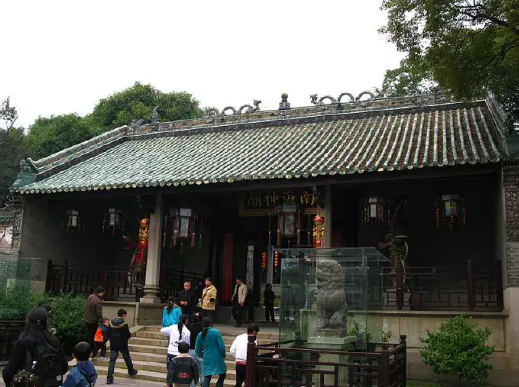
\includegraphics[width=\textwidth]{images/image-29}
	\caption{南海神庙又称波罗庙,位于广州市黄埔区庙头村(旧称扶胥村),是古代皇帝祭祀海神洪圣的场所,也是世界海洋贸易体系东端。南海神庙始建于隋朝开皇年间,至今已有1400多年历史,是桂枝四海神庙中唯一完整保存下来的建筑遗迹。}
\end{figure}

官员怎么看这个地方呢?

“广州边海,旧饶,外国舶至,多为刺史所侵。”(《南史》)

这是官员贪污腐败,外国船进来我就打秋风,粤海关一直到清朝都是这样的。

“经大庾,则清秽之气分。”(《南越志》)

过了大庾岭就是花花世界。

“世云:广州刺史,城门一过,便得三千万也。”(《南齐书》)

到那里就是打秋风的,一个外国的殖民地方,很有钱,贸易港口。

这个就是前半期了。那么我们就要进入到后半期了。后半期的整个南粤史的精神气质是完全不一样的。我们可以看到南粤本土的共同体最后是运用了帝国的话语,他把自己变成了华夏,这非常有意思的一点,而且他变成了最华夏的华夏,等于是一个小华夏,然后形成了现代的粤文明。这是南粤后半期的一个特点。那我们就开始看。

\section{南汉帝国}

后面就是南汉帝国,这是第三个自治的政权。南汉的建国是怎么样的呢?唐末大洪水,黄巢来了广州(879),当时有一个军官叫刘知谦。刘知谦他说他祖上是河南人,但是他的家族在南粤已经住了两代人,那他到底是不是河南人的后代呢?不好说,可能是攀附。有研究表明,刘氏家族很可能是阿拉伯人后代。当时他在地方也算是一个小土豪了,一个将领。他发动自己的宗族、乡党这些人。当然这些人很有可能很多都不是中国血统,很有可能很多是外国人。他们把黄巢打败了。我们看到,这个土豪依靠外来的秩序,本地的蛮族已经不行了,只能靠外国来输入秩序。他养了一万多个兵,就成了割据一方的一个势力了。过了十几年,他挂了。他的儿子叫刘隐,他继承了家业(894)。广州当时有两个帝国官僚都想占据这个地方,叛乱,被他都打平了(896、898)。然后基本上他就控制了岭南(唐昭宗乾宁三年(896年),刘隐出兵奇袭肇庆、广州)。

当时唐朝的控制权,经过黄巢大洪水,已经衰落得不行了。唐朝是907年灭亡的,唐末真正掌握实权的人是朱温,他是华北的大军阀,后来后梁的皇帝,朱温控制了朝廷。当时广州有什么?它是殖民地,有财宝,有各种北佬没见过的东西,刘氏就大量的贿赂朱温。朱温就说好,你就当清海军节度使(904)(895年,岭南节度使改称为清海军节度使。刘隐(901年—911年)任清海军节度使。天祐元年(904年),授任清海节度使),反正我也过不去。907年就变成后梁了。朱温封他为南海王(911),同年刘隐就死了。他的儿子叫刘岩,他在公元917年,因为北方根本管不到他,他就称帝了,然后建国叫“大越”,但是第二年就改成了“汉”,他说我是汉朝的后代,因为姓刘。他改了一个名字叫刘䶮。

\begin{figure}
	\centering
	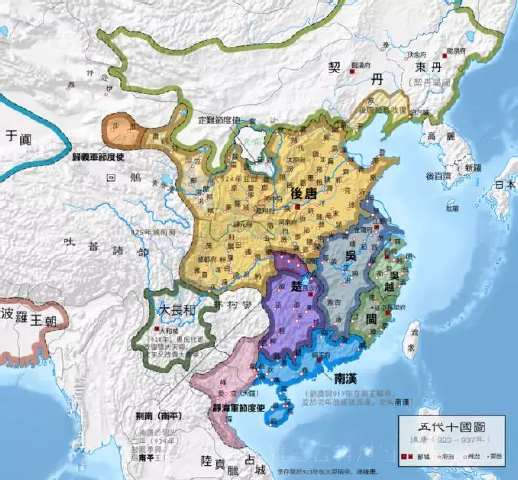
\includegraphics[width=\textwidth]{images/image-30}
	\caption{五代十国图(后唐代:923年-937年)}
\end{figure}

南汉有一个特点,其实它的宫廷是很桂枝化的,因为他们很喜欢攀附,等于说他选择了这个路径之后,他的德性就下降了。刘䶮是高祖,晚年开始他就很奢侈,反正广州这个地方,你想不奢侈也很难。喜欢用各种酷刑。等到他死的时候,他的儿子叫刘弘度,他上台(942)之后干的第一件事情就是要美女跟伶人,到宫里演戏。这个就是典型的支那宫廷的故事。于是他的弟弟刘弘熙,后来改名叫刘晟,就是中宗,他在第二年看到他哥哥不行,然后就发动了一个宫廷政变把他哥哥杀了(943)。杀了之后不要紧,他就怕别人也学他,就把其他十四个兄弟全杀了,一个不剩都杀了(943~955)。不光是把兄弟杀了,把他们的儿子、孙子全杀了。然后这些家族里面的女眷,侄女、嫂子之类的都收到宫里来玩。接着开始大规模地扩张,跟北方的湖南的南楚还有吴越的南唐打仗,争霸战争。我们今天在广东北部能看到很多南汉修的军事堡垒,就是南汉中宗干的事情。这就是一个很典型的支那皇帝了。最后他死了(958),他没活太长,估计也是累死的,这么多美女。

他的儿子叫刘继兴,后来改名叫刘鋹,就是最后一个皇帝,南汉后主。他很宠爱一个波斯女子,他给她起了一个nickname叫媚猪,很可爱的小猪。他也很喜欢用酷刑。而且他非常不放心的就是这些文士和武将,他喜欢用太监。这个时候广州就出现了一种风气,自宫。那些有军事才能和有文才的人都自宫,科举的状元,他就把状元都阉了。当时据说广州城里有二万多个宦官。自宫的人不一定全都能进宫,因为这个是有就业岗位的,等于说你去考公务员,现在是出卖灵魂,那时候是出卖你的生殖器官。所以说这个朝廷是一个很鬼畜的朝廷。

还有一个就是,刘鋹对佛教的信仰是无以复加的。我们看这句话:“崇信释氏教,于府城四面建二十八寺,以应列宿。”(《南汉书·后主纪》)“释氏教”就是佛教,“于府城”就是在广州,四面建二十八座寺,以对应天上二十八个星宿。把广州改名叫兴王府,然后建了不计其数的宫殿,这些宫殿的名字我没有列,因为实在是太多了,数以十计,今天全都没了。园林不可胜计,现在广州有一个遗址叫药洲,那里一个宫苑遗迹,是一个水中的小洲,南汉朝廷在那个洲上面放了各种各样奇怪的石头,皇帝在这个地方求仙、炼丹。这些宫殿并非纯东亚式的宫殿,里面有很多西亚器物。总之,这是一个很迷幻的朝廷。这个就是南汉的特质。

\begin{figure}
	\centering
	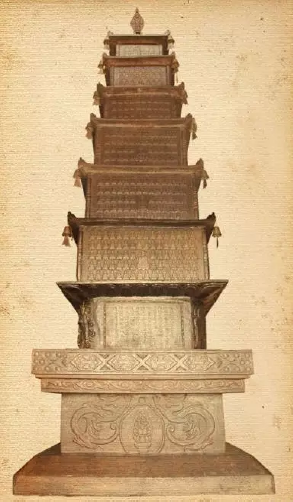
\includegraphics[width=\textwidth]{images/image-31}
	\caption{南汉千佛铁塔}
\end{figure}

\begin{figure}
	\centering
	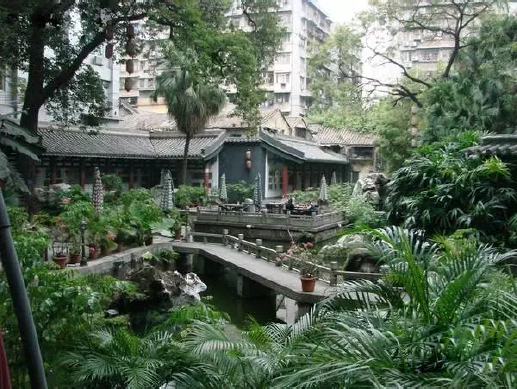
\includegraphics[width=\textwidth]{images/image-33}
	\caption{药洲遗址}
\end{figure}

南汉宫廷能进行这样的生活,一个当然是靠汲取,第二个它靠的是贸易,而且它本身有外国的背景。所以说这一点还是很值得肯定的,就是他对贸易非常重视,他不贸易就拿不来这些东西。他对外非常开放,他是鼓励海外贸易的。而且他跟北边的吴国关系很好,因为他就怕中原的五代真的找他问罪,于是他跟吴国在海岸线上是有很好的贸易往来。当时有一句话叫“结联淮海,航海梯山”,大量的船队在江淮和南粤之间贸易,两边结成军事同盟去对抗中原的五代。有点像东南互保。除此之外他们还招徕外国的商人,因为他们本身就是有外国血统的。他招大量的海商,让这些人到这边来通婚。后来宋神宗,就是所谓的改革皇帝,他说过两句话,说南汉其实不错:第一是南汉“笼海商得法”;第二个是为什么南汉能据守广东一隅呢,因为它“内足自富,外足抗中国”,所以它是可以维持下去的。

但是,我们知道他要维持这个生活要靠贸易,但是最重要的还是靠汲取资源。南汉养了二十万军队,人们的负担是很重的。赋税是很沉重的,汲取得很厉害的,贸易的汲取也很厉害的。但是我觉得还不能光说它是小型桂枝,它有很浓的西亚色彩、海外色彩。当然它也是一个历史节点,如果它没被宋朝灭亡,也可能它最后能走出一条跟桂枝不一样的路径也说不准。它可能会把南粤带入到西亚中亚的秩序、印度的秩序、南洋的秩序中去,那这个历史就完全不一样了,这个历史就很有趣了。

\begin{figure}
	\centering
	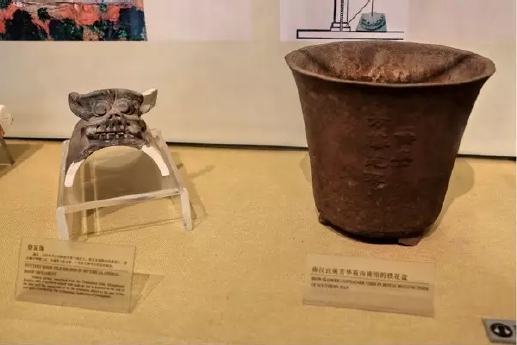
\includegraphics[width=\textwidth]{images/image-35}
	\caption{南汉王宫的铁花盆、鬼脸瓦}
\end{figure}

宋代消解了这种可能。宋太祖是派潘美南征(970),这支军队打得非常的顺利,第二年刘鋹投降,南汉就亡国了(971)。刘鋹其实最后活得还不错,不像南唐后主,估计是知道他没有太大的威胁,他没有太大的志向。南汉残余势力的最后一起起义,发动者是个名叫乐范的太监,这个王朝最后是靠太监,靠这种无产者去做忠臣。因为太监没有别的出路,他只能忠于皇帝。这次起义很快被宋军给剿灭了(972)。于是南汉历史就终结了。这是一个非常有趣的王朝。

\section{第四次北属}

南汉没了,于是就进入第四次北属。这是宋元时代了。宋元时代,广东这个名字就定下来了。宋朝打下了岭南之后设了一个广南路(971),后来到了宋太宗的时候,他把天下分为十五路。广南路在宋朝就分成了东西两路(997),一个是广南西路,一个是广南东路。广南东路的简称就是广东。元代设了一个道叫广东道。明清就是广东省,最后清代就形成了三州十府(连州、罗定州、嘉应州、广州府、惠州府、潮州府、肇庆府、高州府、雷州府、廉州府、琼州府、韶州府、南雄府)这样的一个格局,就是今天的广东了。从宋代到现在,这个疆域基本上是没太多变化了,只有廉州府北海最后是在我朝的时候送给了广西。

南汉是一个节点,是另一种完全不同的尝试,它是卡在中间的一个插曲。北宋就进入了小华夏的建构历程。北宋有一个特点,在北宋,南粤基本上没有发生大规模的叛乱,没有发生帝国官僚据城叛乱的事情。前面是很多。为什么?因为宋朝的地方精英科举士人,他在南粤本土没有太强的根基,这些人就是忠于王朝的,所以当时南粤很少有超过一千人的叛乱,只有一场很大的战乱,就是侬智高之乱(1052~1054),宋神宗的时候。侬智高是一个壮族的豪酋,反抗宋帝国,最后一路打到广东,围攻广州五十七天(1052年6月21日开始围城)。当时本地有一个士人,是曲江人,韶关人,叫余靖,他组织广州城进行了防御,他在地方上是有威望的,守住了广州城。这是一个信号:本地的汉人的士大夫第一次把这个地方当成了自己的家,因为宋朝跟科举士大夫关系是很密切的。

接下来就是帝国的儒化教育。广州知府蒋之奇在宋神宗的时候扩建了一座府学(1087),府学就是地方学校,专门讲儒学的。培养的是什么人才呢?士大夫,为了科举,这些人要学经典。整个宋代,整个珠三角设了一座府学和五座县学,北宋四县(南海、东莞、增城、新会),南宋一县(香山),重要的居民点都有儒家士大夫的培养机器。这是北宋的情况。

\begin{figure}
	\centering
	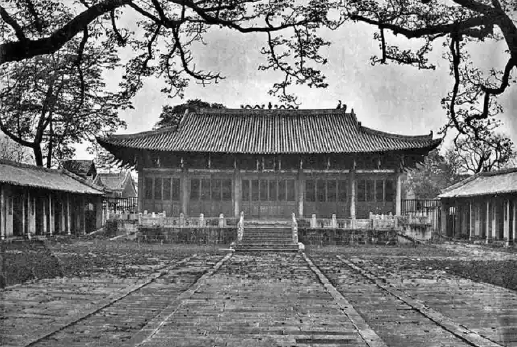
\includegraphics[width=\textwidth]{images/image-37}
	\caption{广府学宫大成殿}
\end{figure}

在宋代,南粤基本上没有太大的战争。两宋之际,金人南侵,靖康之变(1125~1127)。之后在湖南发生了钟相杨幺起义(1130~1135),兵匪在江西和湖南一带活动,并在广东北边扫了一个尾,所以粤北被屠戮得比较惨。基本上广州一带没什么事情,韩江流域也没什么事情。所以说两宋之际的大洪水对南粤的波及有限。

南宋,理学开始试图扎根南粤,于是就开始出现了奉行理学的地方官。我们知道理学的一个最关键的社会改革,是在基层建设宗族,小共同体。氏族什么的已经没了,他要建设小共同体。这个时候南粤就出现了理学地方官,最有名的是朱熹的大徒弟廖德明,他当过广州的知府,第一次刊行了《朱子家礼》(1211)。《朱子家礼》就是一个介绍宗族的指南,等于说后来宗族社会很大程度上是靠这本书起来的。

于是在他们的培养之下,本地人也出现了一批理学高官。这些人到底是出身粤人还是汉人呢?我们已经不清楚了。因为它有这么多培养士大夫的机器,所有人都可以进来的。那么南粤就出现了一个特别大的官,叫李昴英(1201-1257,广东番禹人,治春秋学,广东第一个探花),他在南宋的时候当过吏部侍郎,等于说进到帝国的内圈了。他推行儒家的礼仪,乡饮酒礼,就是每隔一段时间把地方的父老都叫过来先训话,把违反儒家道德的人批判一番,把符合道德的人表彰一番,然后大家一起愉快地喝酒、行礼,就是这样一种儒家的礼仪。他开始在南粤大规模地推行这一儒家礼仪。

\begin{figure}
	\centering
	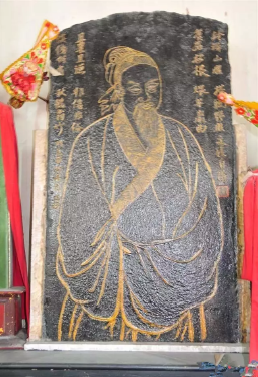
\includegraphics[width=\textwidth]{images/image-38}
	\caption{番禺李公祠内的李昴英石画像}
\end{figure}

宋代理学家是试图在南粤扎下根的。而我们知道南粤,在汉人的城市外面,之前它是粤人的地盘,粤人有没有自己的共同体呢?有的。当儒家、宗族的观念要打进去的时候,一开始肯定是不会太受到欢迎的。这完全是两个组织架构。所以说我们可以看到,宋代在南粤的儒学建设基本上是浮在表面的:在城里这些东西搞得比较好,有一帮人在提出理念;但是地方上没有变。可能会有一些原住民变成理学士大夫,比如李昴英这种人;但是基本上,其实出了殖民点还是另外一个世界。

北方发生大洪水,南粤是一个安全岛。在宋代是有两次大规模的北人南迁:一次是两宋之际的靖康之变(1127年前后),一次是元军南下(1276年前后)。他们走的路线就是大庾岭这条线。我们知道,从江西进到大庾岭,进来之后第一个大的府城是南雄。南雄有条重要的道路叫珠玑巷。一般来讲移民就要从这边过来。于是到了明代就出现了一个发明民族的材料,就是珠玑巷,这个先按下不表。我们知道有大量的人从这里过来了。这些人过来之后也等于说增强了当地汉人的人口和势力,也为后来明代的大规模宗族化、理学化和建设小华夏打下了基础。以上是宋代南粤的历史。

那我们再看一看宋元士大夫眼中岭南的民风是怎么样的:“盖水陆之道四达,而蕃商海舶之所凑也。群象珠玉,异香灵药,珍丽瑰怪之物之所聚也……好义之心,不能胜于欲利,岂其势之使然。”(元《南海志》)

这段首先讲的是贸易,还是很发达的,跟南粤在汉朝以来是一样的现象。宋人认为这是什么现象?认为这是不好的现象。为什么不好?因为不义。我们知道理学跟之前的儒学不太一样,理学是有一种传教的狂热的。因为理学最早是怎么出现的?就是因为隋唐基层信佛信道信得太厉害了,韩愈就开始说,我们要跟他们争夺群众,所以后来才发展出理学。理学是把儒家宗教化了,它把道家跟佛家的本体论抄过来。我们看到,唐代人是以一种什么角度去写这些人的呢?态度有什么不同?唐代人觉得无所谓;但是宋代士人觉得这个风俗是不对的,他们是带着怜悯之心,自作多情地觉得你们这些人实在是太可怜了,你们没有符合伟大孔子跟朱子的教导,你们整天争利而不讲究大义,你们这些人实在太不行了,太低档了,你们不是我们这种优雅的士大夫。

\begin{figure}
	\centering
	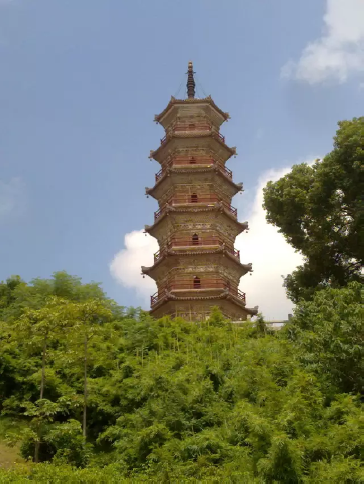
\includegraphics[width=\textwidth]{images/image-40}
	\caption{河源龟峰塔,建于南宋年间}
\end{figure}

“俗喜游乐,不耻争斗。妇代其夫诉讼,足蹑公廷,如其在家室,诡辞巧辩,喧啧诞谩,被鞭笞而去者无日无之。巨室父子或异居焉,兄弟骨肉急难不相救;少犯长、老欺幼而不知以为非也。嫁娶间无媒妁者,而父母弗之禁也。丧葬送终之礼,犯分过厚,当然无制。朝富暮贵,常甘心焉。岂习俗之积久,而朝廷之教化未孚欤?”(元《南海志》)

这是一段元代士人写下的材料,首先是大大批判了一番南粤的风俗,说女人乱来,认为没有宗族的伦理;“嫁娶间无媒妁”,自由恋爱;丧葬之礼又太重了;“朝富暮贵常甘心”,无所谓。他们认为,很可怜啊这些南粤人,需要教化,他们是很焦虑的,这个地方怎么行呢?一定要教化,但是他们教化不了。我们看到,明清之际的南粤对满清的抵抗,要比宋元之际的南粤对蒙元的抵抗激烈得多。因为明代建构出了一个小华夏,对满清是有本能的极大的仇恨的。但对元就打了三年就完了。宋元士人出于狂热的理学传教情怀,对南粤“堕落”的风俗很焦虑,我们能感到他们那种深刻的焦虑感,但是他们没办法。

元军在1276年占领了临安,残存的南宋朝廷就退到了岭南。所谓抗元义士的蜂起都是那些士大夫组织的,他们没有特别强的群众基础,然后就纷纷的都被镇压了。元军是很残暴的,把广州的东城、西城给烧了(1276~1277元军与守军进行拉锯战,广州城破坏严重),把潮州屠了(1278),这些都是汉人聚集的大城市。最后新会崖山海战之后,南宋就灭亡了(1279),这是通史的知识。才三年,抵抗就被粉碎了。

\begin{figure}
	\centering
	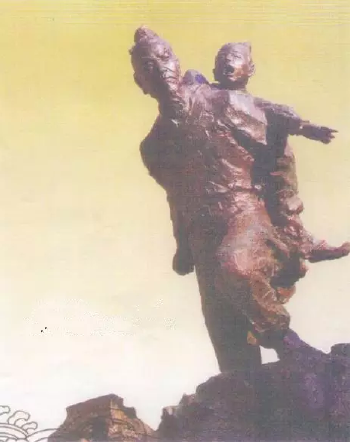
\includegraphics[width=\textwidth]{images/image-41}
	\caption{陆秀夫负宋少帝跳海}
\end{figure}

元代,南粤的儒化运动受到了严重挫折。我们知道,元代的宪制根本就不是儒化的,它有大量内亚的宪制,伊斯兰的宪制和基督教的宪制,干嘛用儒家的呢,儒家的只是拼图不太重要的一块,可以说是一个外围婊。南人的儒士,这些在宋代很焦虑、要教化别人的这些儒士,他们就没事可做了。元代中期的时候才有科举的(1313)。当时蒙古人觉得哪些人跟他感情更好呢?色目人。色目人是什么人?是那些中亚的人,绿教徒还有基督徒,像马可波罗这种人,他觉得这种人反而跟更对脾气,不像那种酸臭的儒家士大夫。十四世纪,大量的这种人就跑到了广州来,还建了教堂。广州的格局还是延续了海外贸易的格局,从南越以来一直是这样。它的贸易一直到了拜占庭,一直到了马达加斯加,都有贸易的路线。进入这条路线的,各国的人都有。还是这样的一个格局。除此之外,佛寺在这个地方非常厉害。我们知道元代的皇帝是很信佛的,当然他们信的是喇嘛教,但是汉传佛教也是鸡犬升天,可以攀附一下,于是他们就占有了大批土地和信徒。珠三角现存的最早的一份土地契约就是元代的:

“广州城南信女郑氏念八娘,同夫居士林伯彰,用铜钱千缗,置龙冈坊蔡天兴土名石砚田、涌底田共八十七亩,又蔡芳田四号,舍入风幡大道场,岁收租利,供佛及僧。”元至元二十四年(1287)

广州城南有一个信女郑氏,叫郑八娘,他的先生叫林伯彰,他们用了千缗的钱,把龙冈坊的一块叫石砚地方的田还有一个涌底田,买了八十七亩的田,又把一个叫蔡芳的人的田收购了四块,把这么大一大块田全部都给了寺庙,让他们做道场,田里面收上来的租子都供寺庙来使用。等于说当时人关心的就是这些东西。这是珠三角最早的契约,就是这样的一个东西。所谓的理学化在这个时候完全失败。广州还是保持着历史上那个隐秘的格局,就是说汉人的殖民点,虽然汉人的人数在增加,但是外面的粤人和外国人的势力跟帝国的秩序是完全不搭调的。按照儒家的观点,宋代曾经试着进行过一次教化,但是没有成功,元代又反动回去了。

\section{何真政权}

在这种社会,土豪非常容易出现,因为帝国的触角并没有深入到太基层。于是我们就进入到何真的历史世界了。就是我写的那篇文章,《死去的南粤骑士:何真》。为什么会有何真?他身上积攒的是从南越一直以来的这样一个传统,就是这种本地的土豪,他对帝国的伦理并不是太在乎。还记得我写的那篇文章中,他说谁杀王成我就给他一万块,那个人杀了,他先把钱给了那个人,很守信,接着又拿个锅把人家给煮了,说“奴叛主者视此”。就是很朴素的一种东西。在儒家看来这太野蛮了。

\begin{figure}
	\centering
	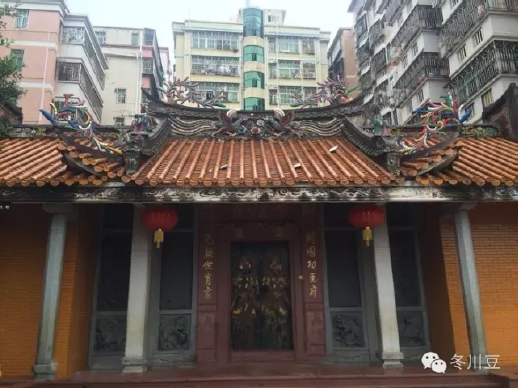
\includegraphics[width=\textwidth]{images/image-43}
	\caption{何公真祠,由作者亲摄}
\end{figure}

我们知道,元朝到了晚年之后也有宪制的斗争,元顺帝相对来书是比较汉化的一个皇帝,元朝的汲取能力也是越来越增强。元末对南粤的税是元初的二十多倍。最早反元的一个起义就是在今天的广州增城爆发的,领导者叫朱光卿(1337)。当然是被讨平了。随后元朝的统治开始瓦解,帝国崩溃了。当帝国这一层外衣退下来的时候,各地土豪的秩序就浮现了出来。于是到了何真的时代,一三六几年的时候,大半个南粤都陷入了土豪割据当中。于是我们进入到了何真的世界。这样大家才可以理解,为什么那时候会进入一种像战国时代的一个面貌。以下是对何真事迹的概括:

\begin{quote}
何氏:东莞大户\\
结寨、集乡兵自保(1355)\\
拯救惠州(1361)、广州(1363)\\
击退陈友谅军;诛宿敌王成(1366)\\
成为南粤之主,拒绝自立(1367)\\
投降明朝(1368)\\
朱元璋利用何真,北迁、杀戮土豪、何真旧部3万余人。\\
何真被明廷封为“东莞伯”,洪武二十一年(1388)去世。\\
五年后,何氏以“蓝党”案被族诛。
\end{quote}

这些其实都不用讲了,我那篇文章\footnote{指《死去的南粤骑士·何真》——Setsuna K}大家都读过,总之他是控制了南粤。在1367年,他控制了南粤,他就是南粤的老大了。他那时候也不投降明朝,也不投降元朝,等于就是一个独立的政权。有人说那你就自立当皇帝,效赵佗故事,他把那个人杀了。因为在他看来,他就像傅作义一样,他觉得跟谁都一样,反正我有这么多人我有这么多地我怕什么呢?于是1368年明军一来就投降了。然后他就悲剧了。这个我的文章也讲过。

\section{第五次北属}

于是就进入了第五次北属,就是明清时代,洪武社会主义,阿姨写过(《朱重八的历史使命》),不多说了。洪武社会主义的一个重要元素就是亚述式的大迁徙,他让何真一次次回到南方,回到南粤,把旧部召集起来打包送到北方,再回、再送走。然后土豪都送走了,就开始编人民公社,以里甲组织控制这些人。再把一部分人编成军户,这些人也是世袭的,建设军队的卫所。这些人都是世袭的,也是不能动的。还有就是打土豪了,我那篇文章里也讲过,何真一些旧部造反,他就把那些人都杀了,杀了一万多人。还有一个就是朱元璋搞的海禁。海禁是一个非常大的摧残,因为从南越和汉朝开始的传统到这个时候已经大概一千五百年了。比如说一个人去汉朝的广州、去元朝的广州,他感觉可能会差不多,都是一种光怪陆离的世界;但这个时候,阿姨就说,朱元璋把元末拼图式的世界变成了一个均质化的世界,这就是洪武社会主义。

\begin{figure}
	\centering
	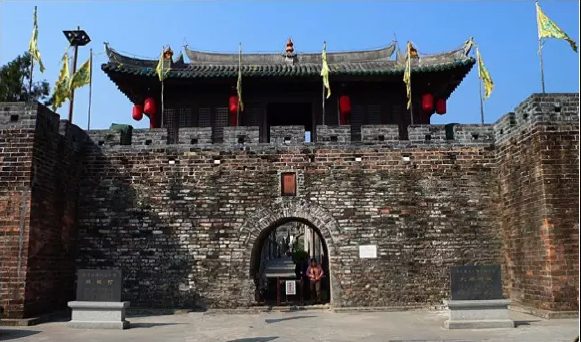
\includegraphics[width=\textwidth]{images/image-45}
	\caption{修建于洪武海禁时的大鹏所城}
\end{figure}

这里有两段材料。第一段是朱元璋的口语诏书,非常好理解:

\begin{quote}
明太祖洪武三年(1370)圣旨:

我这大军如今不出征了,都教去各州县里下着,绕地里去点户比勘合。比着的,便是好百姓。比不着的,便拿来做军。比到其间有司管理隐瞒了的,将那有司官吏处斩。百姓每自躲避了的,依律要了罪过,拿来做军。钦此。(《戒庵老人漫笔》卷一)
\end{quote}

所有人都要编户,扁平化管理,管你是什么粤人也好还是汉人也好,统统给我编户。没有户口的是什么人?不是好百姓,就要拿来做军。控制每一个人。他要设计的是一个什么样的社会呢?我们可以看一下:

\begin{quote}
洪武十四年(1381)立里甲制度:

诏天下编赋役黄册,以一百一十户为一里,推丁粮多者十户为长。余百户为十甲,甲凡十人。岁役里长一人,甲首一人,董一里一甲之事。先后以丁粮多寡为序,凡十年一周,曰排年。鳏寡孤独不任役者,附十甲后为畸零。儒僧道给度牒,有田者编册如民科,无田者亦为畸零。毎十年有司更定其册,以丁粮增减而升降之。册凡四:一上户部,其三则布政司、府、县各存其一。上户部者册面黄纸,故谓之黄册。(《明史•食货志》)
\end{quote}

这是要大兴户口统计,黄册是大型户口本。里甲是什么东西?有一些没有格局感的蛋头学者居然说它是地方自治组织,其实这是人民公社。你看任役的都是一些什么人,里长跟甲首。什么样的人才可以当里长和甲首?有田产的人。而那些没田的人不在这个体系里,他们叫畸零,不用当差。这就是一个人民公社,压榨有产者。每十年要统计一次,为什么要统计一次呢?因为可能会有土地产权的变化,我再重新排排,谁有田了,好,出来,你给我交粮、服帝国的徭役。再过十年之后还是这样。他设计的就是一个这样的世界,不断对有产者进行阶级斗争。所以说有的没有格局感的学者说这个是地方自治,说让富人管理乡间的事务,这根本不是一回事,这就是一个帝国的秩序。黄册就是这样的一个阶级斗争的工具。里长主要是服役,就是交粮。比如说朝廷说要交粮了,你就要下去收税。但是其实经常收不上来税,就得你自己交,不交要充军的。朱元璋就是一个下等人,对土豪是有一种本能的阶级仇恨。王安石都没有到他这一步,王安石只是国家贷款给农民。

\begin{figure}
	\centering
	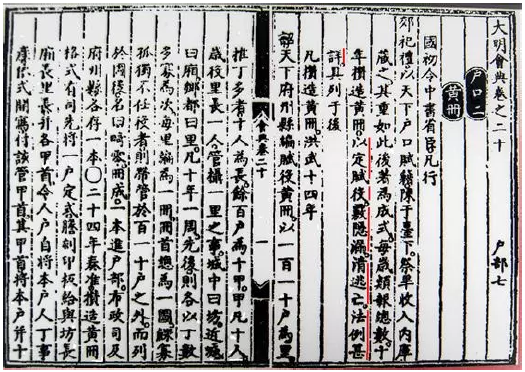
\includegraphics[width=\textwidth]{images/image-46}
	\caption{《大明会典》(万历内府本 共228卷) 记载:洪武十四年(1381)诏令天下府州县编赋役黄册。“以定赋役、覈隐漏、清逃亡。”}
\end{figure}


儒家有一个缺陷,就是不患寡而患不均,但是如果真出现朱元璋,他们又害怕,真的来了。这个就是前所未有的帝国的统治,涉及到了每一个人,无所逃于天地之间,大家都加入人民公社。当时里甲出去是要有路引的,就是介绍信,跟毛时代是一样的。而且很有意思的是,朱元璋要让大家背他写的那个大诰,背朱元璋语录。在洪武十九年,他从天下召了十九万个读大诰读得最好的人,到南京来,接见他们,就像毛泽东一样。后来他还命令,看到哪个地方胥吏欺压百姓,百姓就把他抓到南京来,类似文革。毛泽东玩儿的东西,他六百年前都玩儿过了。

这个体系在十四世纪是不可能维持下去的,因为社会是在变动的,他不可能有毛时代的那种控制方法。毛时代有铁路,有电报,有飞机大炮,老百姓造反,根本打不过,大跃进那些人造反怎么样?都被机枪给突突突了。这种社会是根本就不可能维持下去的。最后这个社会一变动,这个体系就要崩溃掉了。于是在明代中期,社会出现了大量的流民。老百姓受不了只能跑,土豪也没有了,你没有人能依附,你就只能跑。于是明代中叶,整个社会都已经陷入一种解体的状态。大规模的流民暴乱到处爆发,在帝国的各处都在爆发,整个社会就进入一种小洪水的状态。

所谓广东的黄萧养之乱,就是我写的那篇文章《南粤土豪的胜利——1449年佛山血战》写的故事,我就不仔细讲了。黄萧养在1448年,也就是土木堡之变爆发前后造反,打了一年多他就挂了,那些流民也比较缺乏战斗力。很重要的就是佛山,因为这个地方比较特殊,这个城市是自发秩序形成的,地方自治的传统比较坚实,所以朱元璋没有把他们太怎么样。他们是披上了里甲的外衣,土豪是整族整族地进入了里甲,其实毛时代也有这样的事,广东好多的人民公社就是宗族换了一件衣服。南粤一直有一个特点,哪怕是这种社会主义,也很难完全控制住,因为太远。毛时代也没有完全控制住。

\begin{figure}
	\centering
	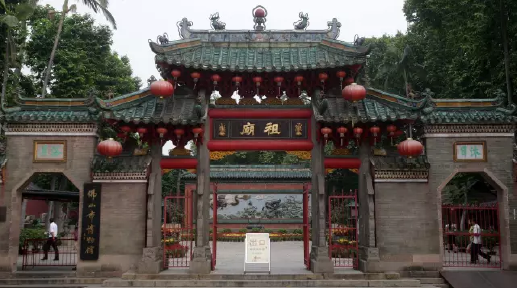
\includegraphics[width=\textwidth]{images/image-48}
	\caption{佛山祖庙}
\end{figure}


\begin{figure}
	\centering
	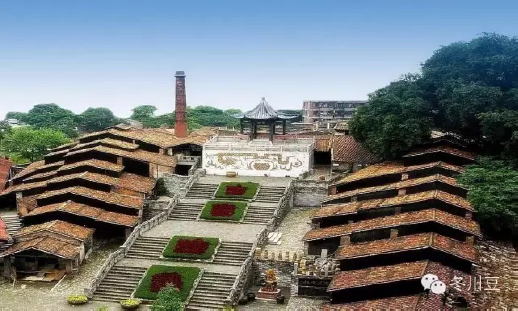
\includegraphics[width=\textwidth]{images/image-50}
	\caption{南风古灶}
\end{figure}

佛山是一个很特殊的地方,我这个文章也讲过,因为它在广州西面,从西江过来的广西的货物一定要经过它,它的经济非常发达。在宋元的时候,它通过贸易形成了一个大镇,那些人在明初又搞冶铁业,变成大土豪。明初也没有把这些大土豪怎么样,他们把自己打扮成里甲,最后打了这场佛山战役,佛山“二十二老”盟誓祖庙,抗击黄萧养。除了佛山之外,南粤还有一些小的土豪。明朝发现,因为它的洪武社会主义崩溃,它的军队根本没用,它的军队好多都逃了,那些部队主要就是靠这些土豪在打仗,它最后就不得不靠这些土豪来给它收拾残局。打完之后,地方社会就进行了重新的整合,虽然还是编户,但这些编户的意义不一样了。

黄萧养造反的地方就是顺德,这个时候设了顺德县。顺德县是谁设的呢?不是朝廷设的,是当时地方一个聚众自保的大户,叫做罗氏,他跟朝廷说,我们来设顺德县,说“治以官司,联以户口,齐以科教”。我们想想,为什么他要让朝廷设县?为什么一个土豪居然会要让朝廷来控制自己?因为不能正面对抗就来迂回。朝廷也没办法,朝廷控制不住了,那就只能我们都来演戏,你来假装你是朝廷的顺民,在地方上自治,不威胁到朝廷就可以了。于是就用这种方法开始走向了小华夏的路线。

\begin{figure}
	\centering
	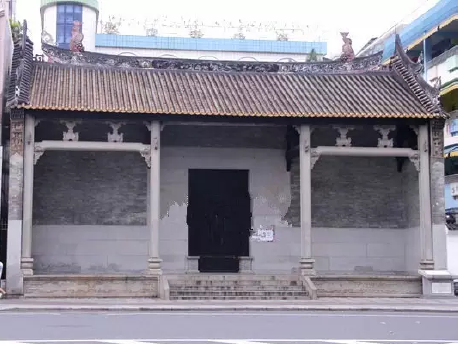
\includegraphics[width=\textwidth]{images/image-51}
	\caption{顺德罗氏大宗祠遗址}
\end{figure}

最早进行小华夏尝试的是新会。珠海再往西是江门,就是新会那个地方。新会那个地方再往西,山区里面有瑶族,当时跟瑶族在打仗的。当时县城有一个地方官,二把手,叫陶鲁(?~1498),他是广西粤语人。其实一般来讲,帝国是不喜欢让本地人当本地官的,因为这样怕你造反。陶鲁在新会先后担任县丞、知县,很有威望,曾团结全城土豪、率领全城百姓打退了瑶人的进攻,复制了一场佛山击退黄萧养之战,他是一个土豪化的地方官。陶鲁后来率军在粤西和瑶人作战,所到之处到处设立培养儒家士大夫的县学。他是本地人,他为什么要拿帝国的意识形态去教化本地人呢?因为这对本地人是有实际好处的:因为其实这只是一个土豪自治的变相,本地土豪进入帝国体系中去后,更多的本地人可以得到庇护,用帝国的话语去让自己的土豪行为合法化了。

另一个就是,他庇护了一个人叫陈白沙(1428~1500)(参见作者另一篇文章《南粤小华夏的种子播撒者:陈白沙》),这是明代思想史最重要的人物之一。三个人,陈白沙、王阳明和湛若水。王阳明是吴越人,陈白沙跟湛若水是南粤人。因为宋明理学到这个时候已经有一个变化,就是说,朱子说我们要不断地格物,不断地追求外在的意义,但是格来格去格不出什么,最后陈白沙说我们应该静坐,学问应该自得,不能一味外求。他是引用了佛教禅宗的思想元素,开创了心学。他等于说是王阳明的一个先导。于是南粤理学在陈白沙之后大盛,因为他是江门人,以江门为中心开始大盛。这就是很有名的江门学派。明代的儒学,南粤可以说是重镇。

\begin{figure}
	\centering
	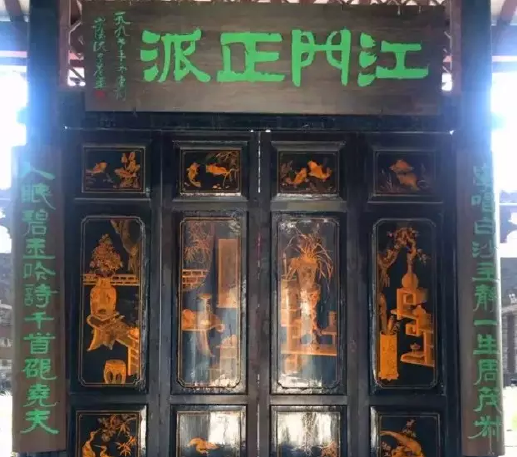
\includegraphics[width=\textwidth]{images/image-52}
	\caption{陈白沙在小庐山设馆教学,并创立“江门学说”,开岭南明儒心学先河,“江门学说”以道为本,以自然为宗,注重“学贵自得”、“学贵知疑”,也被誉为 “圣道南宗”、“江门正派”。}
\end{figure}

陶鲁的行为等于说,我就用这种帝国的手段,让南粤土豪合法化,让我的人进入到帝国的话语体系里;而陈白沙,自己是一个很纯粹的儒者,他相信我就是儒家。因为阿姨说过,发明民族的人,最厉害的人是不觉得自己在发明民族的。陈白沙并不觉得自己是在创新,他觉得我就是真儒家。陈白沙的徒弟张诩给他写的行状说了什么?说我老师祖上是河南人,他生下来普通话说得就很标准,类中州音,说河南话,说他长的也像中州人,不像广东人。但是我们能认为这个是攀附侉子么?这不是攀附侉子,这是一个很微妙的不同,这是一种策略。其实他这个行为是用帝国的话语给自己确立一种合法性,给自己的这种实质上的土豪自治确立合法性,而他又恰恰正好相信我就是华夏文明的真传。而确实我们从实际上看,他也是华夏文明的真传。宋儒乡治主义理想中,华夏文明的本来面目就是这样的一种小共同体林立的社会形态。于是演戏,演着演着就演真了,于是南粤就成了小华夏,虽然陈白沙可能就是一个越族的后人。所以说这个才是民族发明学的奥义,我硬生生地发明出了一个小华夏。我觉得这个是南粤史上最微妙的一个转变,也是最关键的一个转变。

\begin{figure}
	\centering
	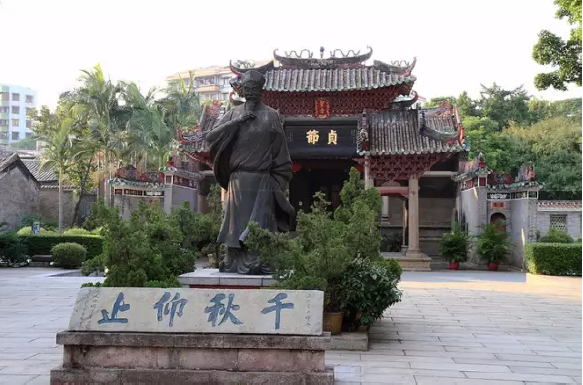
\includegraphics[width=\textwidth]{images/image-54}
	\caption{陈白沙祠}
\end{figure}

再往后就是有人进到北京朝廷的核心了。我们知道,嘉靖朝有一个大礼议,这是明朝很重要的一个政治事件。嘉靖是上一个皇帝正德的堂弟,因为正德没儿子,嘉靖是在湖北的一个藩王,被叫去北京继位的。然后北京那些官僚就想控制他,说你要认正德的爹做爹。于是嘉靖就跟他们撕逼,撕逼了几年,最后打了一批人的屁股,打死了十几个人,这个事情才结束。嘉靖本人肯定斗不过这些理学士大夫的,他是要有弹药的。于是有五个人就站在了他这一边:大家可能看过《明朝那些事儿》,有张璁、桂萼、席书、霍韬、方献夫。后面两个人有一个共性:霍韬是佛山人,方献夫是南海人,他们都是粤人。霍韬和方献夫有一个非常要好的朋友,叫湛若水,增城人,是陈白沙最喜欢的学生。在大礼议前夕,湛、霍、方三人曾在南海县西樵山建书院、讲学、教育宗族子弟、往来切磋儒学学问,在那里建设儒学共同体。霍、方的学问,也受到了陈白沙、湛若水不小的影响。为什么霍、方这两个粤人反而会支持嘉靖?这与陈白沙开创了心学的传统有关,心学本身其实是带着游士性质的,它不像理学,心学强调唯意志论,受心学影响者比较容易出于主观意志、为了自己的利益产生投机心态。

接着又发生了一件事。虽然说已经有这种尝试了,但是其实地方上的信仰还并不是儒家信仰。在帝国官僚看来,在宋明理学的眼中,我们看到宋代士大夫看到那种所谓邪恶的信仰,他们是很焦虑的。于是这个时候南粤发生了一件事,类似于儒家的文化大革命,这个事情叫打淫祠运动(1521),这个是跟大礼议同时发生的。当时的广东提学官,叫魏校,他也是一个很著名的理学家,他发动了毁淫祠运动。我们来看一下他这个运动是怎么搞的:

“照得广城淫祠,所在布列,扇惑民俗,耗蠹民财,莫斯为盛。”(《庄渠先生遗书》卷9)

“淫祠”是什么?按照基督教的话语就是异端思想、异端崇拜。

\begin{figure}
	\centering
	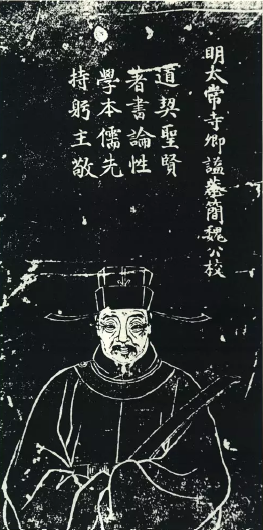
\includegraphics[height=\textheight]{images/image-55}
	\caption{魏校石刻像}
\end{figure}

“社学教化首务也。久废不修,无以培养人才,表正风俗。当职怵然于衷,拟合就行,仰广州府抄案委官,亲诣坊巷。凡神祠佛宇不载于祀典,不关风教、及原无敕额者尽数拆除,择其宽厂者改建东、西、南、北、中、东南、西南社学七区,复旧武社学一区。仍量留数处,以备兴废举坠。其余地基堪以变卖,木植可以改造者,收贮价银工料,在官以充修理之费。斯实崇正黜邪举一而两便者也。”(《庄渠先生遗书》卷9)

说这些东西蛊惑人心,儒家的社学没有搞起来。“不载于祀典”,“祀典”就是朝廷的祭祀典制。哪些信仰和宗教行为合法、哪些不合法?按照魏校的观点,不写在里面的那就是不合法的、邪恶的,这些东西往往是非儒家的。“敕额”就是朝廷给的牌子,比如说朝廷写一个“这个东西好”“这个是个好祠堂”“这个是个好神庙”,那就可以,不好那就是淫祠。然后把这些拆了以后变成社学(县学再下一层的就是社学)。他很有生意头脑,他说把这些拆掉了的材料拿下来卖钱。卖给谁?可以提示一个观点,他跟霍韬、方献夫那些人关系非常好。他就是卖给那些人。而那些人就拿那些买过来的淫祠,本地的士大夫开始建造书院、祠堂。形成了这样的一个关系。

我们今天在珠三角能看到一些遗址,基本上都写的是在这一年被毁掉的。景点介绍上面会写,这个遗址1521年之前是一个什么什么奇怪的庙,这一年就没了。这就是一场,我们可以看成是拜占庭的那种破坏圣像运动。这是南粤历史上非常大的一件事情,整个信仰被转变了。一般讲南粤通史的不太注重这个事,我觉得这个才是历史的草蛇灰线,这个才是一种宪制的改变。

\begin{figure}
	\centering
	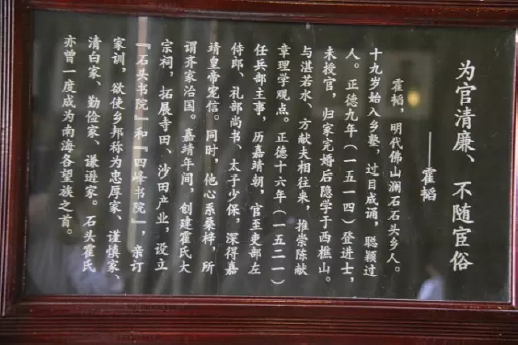
\includegraphics[width=\textwidth]{images/image-56}
	\caption{佛山孔庙中的霍韬简介}
\end{figure}

霍韬(1487~1540,南海人)的宗族是建得非常严密的的,后来明代的宗族化运动中相当多人是拿他这个宗族做模板的。那么霍韬的理学思想是哪里来的呢?前面讲过了,他是在入仕之前,在正德末年,就是嘉靖上台之前,他跟湛若水和方献夫在佛山的西樵山讲学。他们三个人就是讨论这些东西。西樵山很漂亮,大家可以去一去,有很多他们三个人的遗迹,但是很多是后人攀附起来修的。后来还有一个人也在西樵山,康圣人(康有为),当然我觉得他对南粤的宪制影响不大,我都没有讲他。这三个人相对不太受关注,但是我认为这三个人对宪制的影响远远大于那些表面上的人物。他们三个人在这个地方建设共同体,建社学,把自己的宗族都搬过去,搞儒家的共同体,就是恢复理学家设想当中的三代之治。那个地方也是很漂亮的。

他们又参与了大礼议,因为如果你随便一个士大夫就搞宗族,这个还是有危险性的,等于说聚众搞一些朝廷控制不了的事,但是他们就可以大搞了,没人管了,因为他们已经站在帝国权力的核心。很多南粤士大夫也可以搞宗族化运动,因为霍韬、方献夫他们在朝廷中获得了宫廷斗争的胜利,那么粤人在帝国的政治中就产生了影响力,他们搞这个,朝廷不太管了。霍韬参加完大礼议后又在朝廷做了一段时间的官,回粤以后就专注于宗族事务。他编的《石头霍氏族谱》,这个是后来很多族谱的一个模板。其实之前有少量的宗族是有族谱的,但他这个是非常详细。

宗族事务主要四方面的内容。第一个是建祠堂,要祭祖。而祠堂是什么东西?我们知道,桂枝传统社会有没有财产长子继承制?在秦政以后就式微了,变成“诸子分产”。而日本跟朝鲜一直是有嫡长子继承制的,那些次子就很惨。所以我们看到昭和日军为什么会比明治日军的德性差这么多?因为就是很多次子、三子活不下去了,大量进入军队。而长子往往都是有家业的。但是这个就是封建秩序的一种表现。而桂枝是,老人死了,一堆儿子就开始分产,没了,所以说它很难形成一种真正的持久的土豪。商鞅就说,兄弟不能同产,必须要分开。宗族等于是做了一个补救。我要养祠堂,那我肯定要钱,那么我就划出一片田,这片田是谁也不能动的,这片田就是我们的公有财产,我们共同体的公有财产,我们靠这块田上面的盈利去养祠堂、去搞宗族事务。等于说他们用这种方式修正了秦政规划的基层社会。然后第二个,这种财产就可以经营手工业和商业,那么这个其实就有一点像家族企业。所以我们现在能看到,南粤很多企业就是家族企业,就是这种传统。还有第三个,武装自卫。有洪水来了,我们就打仗自保。

\begin{figure}
	\centering
	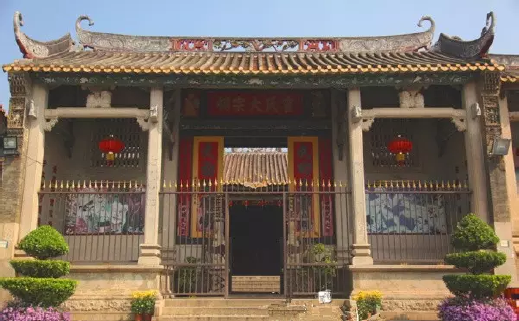
\includegraphics[width=\textwidth]{images/image-58}
	\caption{霍氏大宗祠}
\end{figure}

还有第四个就是发明祖先,我们搞这个东西,我们才是真正的华夏,我们的祖先是河南来的,我们的祖先是从河南、山东之类的地方到了江西再走南雄珠玑巷。于是就发明出了一个故事叫珠玑巷神话,基本上广府60\%~70\%的宗族说这个故事。说宋朝的某个皇帝,没有说哪个皇帝,有一个妃子犯罪了——她和南雄珠玑巷的一个商人私通。珠玑巷的居民怕被牵连,于是大批南逃——而这些居民的祖上也都是历代为了躲避战乱逃到珠玑巷的北方人(往往是历史上的高官),不是本土百越。最后他们逃到南粤腹地,朝廷就不杀他们了。他们就跟地方官说,我们要留在这里,我们要编户口。宋朝的地方官说,好,你们留下来吧。于是这些北方移民后代就留了下来。而且这个故事编得非常像,官方给的文书都编出来了,很多宗族都会写这种东西。但是霍韬其实没有采纳这个。霍韬说,虽然时人都认为自己的祖先是珠玑巷移民,但我不相信这个说法。当然,珠玑巷传说也有一些变体,比如说我见过一家姓赵的宗族,他们说他们是宋太宗的后代,而他们的族谱是什么时候修的?他们是晚清修的。他们其实很可能是客家人,从他们整个的语言和风俗来看。但他们说我们是宋太宗的后代。

这种民族神话有一个什么作用?凝结的作用。我们都是真正的华夏的后代,我们是真的河南人的后代。那些北方的河南人已经堕落了,他们被蛮族和费拉占据了,我们是真河南人。大家明白这个隐秘的关键在哪里了吧,这才是它的关键所在。不是说攀附帝国,这绝对不是,这我要强调很多次。这个就是一个很隐秘的小华夏的路径。而且你发明了民族的神话,那么民族发明的工程便开始启动了:我们就是正统的华夏,我们跟北方不一样。他们用这个手段,真的建造了一个小华夏,上古的华夏部分地在广东复活了。

\begin{figure}
	\centering
	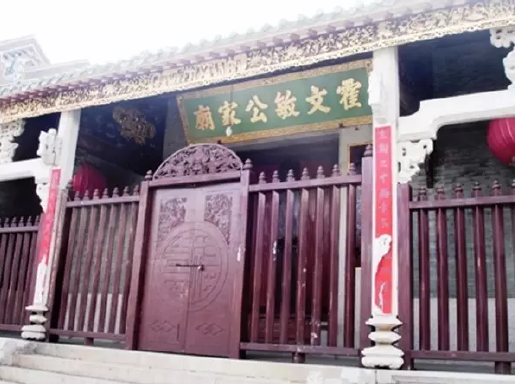
\includegraphics[width=\textwidth]{images/image-59}
	\caption{霍文敏公家庙}
\end{figure}

\begin{quoted}
某听众:湖南也有非常多的祠堂,不知道他们是不是也是认为我是真华夏。福建、江西地方应该也都是有很多的祠堂,宗族势力非常强大。

执经生:不过福建往往是跟神庙结合的,它没有那么儒家,它是更野蛮的一种生长。湖南跟江西,它的宗族似乎不如南粤强大。而吴越因为受到太平天国战争破坏,宗族比南粤衰弱,尤其北吴。可以说南粤的宗族是最成熟的,它的路径走得最好。
\end{quoted}

我们看一下屈大均(1630~1693,番禺人)。屈大均是清初的一个义士,他是一个大才子,但是他不仕清,他觉得你们是夷狄,我是华夏。他在清初看到的南粤是一个什么样的社会,大家看看:

“岭南之著姓右族于广州为盛,广之世于乡为盛。其土沃而人繁,或一乡一姓、或一乡二三姓,自唐宋以来,蝉连而居,安其土,乐其谣俗,鲜有迁徙他邦者。”(《广东新语》卷17)

\begin{figure}
	\centering
	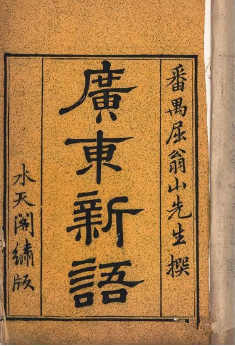
\includegraphics[width=\textwidth]{images/image-60}
	\caption{屈大均所著的《广东新语》}
\end{figure}

这个时候他看到的广东,到处都是土豪,宗族社会发达。而且一个村就是几个姓。为什么会这么同质化?因为他们原来可能就是粤人的共同体,就是一个家族,他们用的汉姓。他说唐宋以来我们就是这种世家、著姓右族,这个是对的么?不对。但是他相信不相信这个?相信。所以说他是最真诚的民族发明家。

“其大小宗祖祢皆有祠,代为堂构,以壮丽相高。每千人之族,祠数十所;小姓单家,族人不满百者,亦有祠数所。其曰大宗祠者,始祖之庙也。庶人而有始祖之庙,追远也,收族也,追孝也。收族,仁也。匪谮也,匪谄也。”(《广东新语》卷17)

这个说的是每个家族都有祠堂,而且他们还要竞争说我的祠堂更厉害。还有大宗祠,大宗祠是始祖之庙,它可能是共同发明一个祖先,比如说我姓陈,他也姓陈,甚至可能我是广府人,他是客家人,我们发明一个大宗祠,因为我们有利益共同体,然后就会有一个始祖之庙。而这个始祖一般是什么人呢?一般都是北方人,都是中原人。这就是发明祖先,发明宗族,只用了一百年时间,屈大均看到的。在宋代的那些理学士大夫觉得非常的棘手的这些社会,一下子就变成这样了。你可以说这个社会就是一个小华夏,宋儒乡治主义回向三代理想部分地实现了,虽然没有封建,可能跟魏晋的氏族比也要差一点,但是基本上这种儒家小共同体,朱熹的理想在南粤复活了,实现了。

\begin{figure}
	\centering
	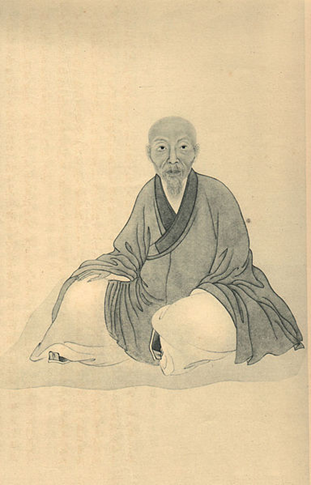
\includegraphics[width=\textwidth]{images/image-61}
	\caption{屈大均晚年像}
\end{figure}

过去的土族到底是一个什么社会形态我们也不清楚,我们只能从汉人的角度去看他的东西,可能那个时候他们也有自己很复杂的宪制我们不知道。我们知道的是,那个宪制在帝国看来是不合法的,他是不断被汉人屠杀和压迫的;而这个时候是“合法”了。而现在有一种观点,说为什么广东都是汉人,是因为汉人把土著给杀光了。是这样么?不是。这些人有汉人也有土著,他们自己都说不清到底谁是汉人谁是土著,你可能只能测一测y染色体才知道父系的情况。而这又涉及到一个观点,到底O1多O3多,你觉得这个重要么?完全不重要。重要的是,你认同了这个东西,你就是真正的小华夏,就是南粤。其实O1也好O3也好,这真的不重要,它等于是相混之后混出了这个东西。清初,这个理想实现了,于是他们对华夏有极大的认同感。他们真的保卫乡土,对清军进行了极其激烈的抵抗。

我们知道,北京1644年沦陷之后,南明先是在南京有一个政权;史可法拥立的南京政权over了,福州有一个政权;福州政权over了,在广东有两个政权。一个在广州,叫绍武政权(1646年12月~1647年1月);一个在肇庆,叫永历政权——就是永历皇帝,流亡缅甸的那个。这两个政权被清军很快灭掉了,它们就是两个帝国的外来的政权。

而这个时候本土的三个士大夫就出现了,广东三忠,他们是非常非常壮烈的:张家玉、陈邦彦和陈子壮。张家玉是东莞人,他在流寇打进北京的时候,他是一个机会主义者,因为跟他没什么关系,李自成抓到他的时候,李自成说你投不投降,他说我不投降,李自成说你不投降我就杀了你爸,但是他爸在东莞,然后张家玉就演戏一样跪下说,好,我投降。后来李自成完了,他就趁乱跑回了老家。等到清军一来,他马上就组织起义兵,组织东莞跟新安——就是深圳的义兵,进行大规模的抵抗。陈邦彦是谁呢?陈邦彦是屈大均的老师。陈邦彦的儿子叫陈恭尹,他跟屈大均并列为岭南三大家。还有一个陈子壮。总之都是一等一的人杰。

他们组织乡民进行了抵抗,围攻广州,最后一个接一个地殉难了。他们对于剃发这种行为是非常的反感的,要维护他们心目中的华夏文明。陈邦彦是被凌迟,陈子壮是被大锯给锯死了。张家玉,他先在东莞打败了,到深圳的西乡,清军追过来在西乡把他打败,然后杀了他的很多人,他逃到增城,最后败了他就投水了。非常壮烈的三个人,广东三忠。

后来清朝在南粤的将领又反了,又据守广州。清朝派了尚可喜过来,搞了一场大屠杀,就是这个广州大屠杀(1650)。各地都是大规模的反抗,反抗到一六六几年还有义兵,反抗了十几年。清军屠了潮州跟南雄。当时,南粤沿海百姓和郑成功进行贸易、有勾连。清朝最后就采取了迁海政策(1661~1669)。广州大屠杀在粤人的心里是一个非常残酷的事情,在粤人心目中留下了比元代的那几个屠城更深刻的记忆。大家先看一看当时的一个传教士写的东西,看一看广州大屠杀是何等残暴:

“大屠杀从11月24日一直进行到12月5日。他们不论男女老幼一律残酷地杀死,他们不说别的,只说:杀!杀死这些反叛的蛮子……最后,他们在12月6日发出布告,宣布封刀。除去攻城期间死掉的人以外,他们已经屠杀了十万人。”——卫匡国《鞑靼战记》

当时番禹县有一个大才子王鸣雷,他就写了一个祭文:“血溅天街,蝼蚁聚食。饥鸟啄肠,飞上城北。北风牛溲,堆积髑髅。或如宝塔,或如山邱。”

这件事情是被记得最详细的一次大屠杀。为什么之前本地人不太记这些屠城呢?很大程度上是因为,现在本地粤人读书的越来越多、华夏化得很厉害,他们觉得这些城市是他们自己的家,而不是简单的帝国殖民点。尚可喜把尸体放在广州东门外烧,烧成一座大塔,十几万个人,那个塔到鸦片战争的时候还在,一个白塔。非常惨烈的一件事情。

\section{海通时代}

所谓的北属时代一直到现在,我认为北属时代还有一个最伟大的时代,就是海通时代,阿姨说这个是最重要的时代。但是因为今天是讲整个的格局,所以说海通时代我就不细讲了,如果细讲可能能讲两、三个小时,我们只是大概过一过海通时代。海通时代是属于第五次北属时代的。它的开始,是西方人来到了南粤。因为到了十六世纪,基本上大航海时代已经来了。最早来到南粤的就是葡萄牙人,葡萄牙人1517年在南粤登陆,他登陆的地点在今天香港的屯门。后来他又跟明朝交涉,他到哪里交涉呢?到南头城,就是深圳的南头城,就是那个南头古城。跟明朝官员交涉以后,明朝官员把他送到了广州,广州当局又把他送到了南京,因为当时是正德皇帝,正德皇帝他正在南方巡游,就见到了明朝的皇帝。然后葡萄牙人又把澳门给借了下来(1557)。我们也可以看到,后来打南明的时候,南明是请了三百个葡萄牙兵,守住了几万清军进攻桂林的这个事情。

明朝灭亡之前,西班牙人、荷兰人跟英国人都到了南粤,清初法国人也来了。在这样的情况下,教会就进来了。最早的一个传教士是方济各•沙勿略(1552),他是耶稣会的。沙勿略是最早把基督教带到日本的,他先在日本传教,他觉得日本这个市场人太少,中国这个才大,于是他到了南粤。但是明朝不让他入境,他说我就算死也要把主的恩典带给中国,最后他是卡在珠江口岸的一个岛,叫上川岛,得了重病,他也不走了,最后就在那里归真。四百年,他的尸体没有腐烂,被教会收藏着,栩栩如生。他是把福音带给日本的人,也是为了把福音带给中国鞠躬尽瘁死而后已的人。下一个传教士就是罗明坚(1583),罗明坚带着一个徒弟,就是利玛窦。他们是采取了另一种方式,他们伪装成和尚,因为佛教不管怎么说在中国是一个合法的宗教。于是就进来,在肇庆建了第一个天主教堂——仙花寺,这是1585年。这个是教会的力量,它让南粤认识到了世界。

\begin{figure}
	\centering
	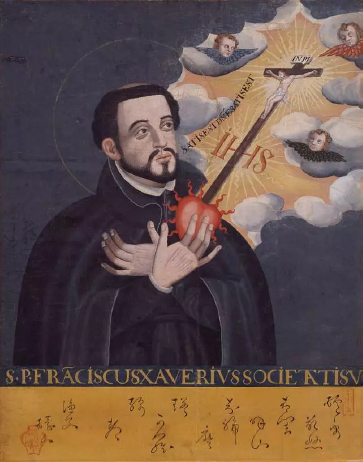
\includegraphics[width=\textwidth]{images/image-62}
	\caption{圣方济·沙勿略画像,日本神户市立博物馆}
\end{figure}

\begin{figure}
	\centering
	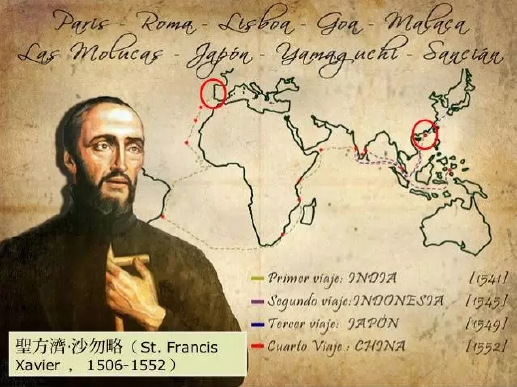
\includegraphics[width=\textwidth]{images/image-63}
	\caption{圣方济·沙勿略}
\end{figure}

还有一个就是海盗的力量。我们知道海通进来以后,西方人会输入火器还有贸易。明帝国是海禁的,那这些人肯定就要冲破你的牢笼,而且当时还有日本的海盗和日本的贸易。到了十六世纪,在南粤本土在进行宗族化的同时,南海的局势大变,等于说西方人直接已经来了,于是海禁的牢笼就被冲破了。很多人就被当成海盗,明帝国说他们是海盗,其实这些人就是海商。十六世纪后半期最大的三个海商都是潮汕人,张琏、林道乾跟林凤,这三个人都非常非常厉害的。戚继光、俞大猷是所谓抗倭名将,抗倭战争最后的一场大战役就是剿灭潮州海盗和倭寇(1561、1562),他们在那个地方屠杀了四万五千人,把这个给镇压下去了。明帝国就是一直在绞杀这些人。

清初的迁海(1661~1669)就更厉害了,这是帝国的另一次绞杀。郑氏集团是一直要奉明,他是在闽粤边界的,他既有闽人的性格又有粤人的性格;但是他作为一个海上集团,他本来应该完全脱离桂枝的体系。但是他没有,所以说他是一个很矛盾的集团。但是不管怎么说,他给沿海制造了一种贸易的可能。而清朝为了防备他,因为他总是跟沿海沟通,于是在1661年下令迁海。这是一场巨大的灾难。当时下的命令是这样的:从山东到广东,所有沿海三十里内的人三天之内要搬完,不搬完的话军队就要屠杀。很多人带着财产就跑了,这里本来是有很繁荣的海上贸易的,这些人就走了,房子就没了,船被烧了,很惨。只有澳门没事,澳门是有西方的秩序,清朝动不了它,不敢动它。其实北方执行的不严厉,吴越、山东不严厉,因为离郑成功远;主要就是福建跟广东,执行得非常严格。

\begin{figure}
	\centering
	\includegraphics[width=\textwidth]{images/image-64}
	\caption{香港周王二公书院:康熙四年(1665年),两广总督周有德及广东巡抚王来任上疏力陈迁海令对广东地区造成六大害,至康熙八年(1669年),清廷批准复界及容许居民回乡居住。香港元朗锦田乡民专门修建书院以示纪念。}
\end{figure}

等到1665年才有地方大员说,不行,老百姓活不下去。因为这些人是靠海吃饭的,你把他们都赶出去,他们吃什么,饿死,内地的人也不喜欢他们,就饿死了。葛剑雄的人口史说广东在迁海当中是死了九十万人,福建死了一百多万人。这是一场巨大的灾难。后来复界的时候,当时新安县——就是深圳的损失差不多一半,损失了四成人口。而回来的时候好多人口都不是本地人,是客家人,客家人占了便宜,就把这些地方都给占了,把深圳东南部给占了,本来这些地方都是广府人的地方。当时是有很多人跑的,其实迁海也就是八年,不像明朝,明朝是一直给你海禁,直到晚明才开了一个口子。1680年,尚可喜的儿子尚之信在三藩之乱中被康熙帝讨平,平南王尚氏在南粤的统治结束。我觉得尚氏肯定不是代表本土利益的,他们是外来的,屠杀粤人,被干掉了活该。

消灭三藩后,清朝就设了四个海关,四口通商,就是江、浙、闽、粤(1685),粤海关就在广州。到了乾隆的时候,1757年,就变成广州一口通商。而这个一口通商其实是帝国控制之下的,你只能跟朝廷指定的这些商人贸易,这些人叫行商,十三行。当然不是十三家商号,在历史当中,数量一直在变,有的时候十六家、二十家都有,少的时候就八、九家。十九世纪一个最大的行商叫伍浩官,他是有三千万两白银的资产,一两是等于六百块钱,据说他是当时世界上最富裕的人,一个广州人。在当时,广州的西方色彩又是很浓厚的。我们就看到,那个有异域色彩的广州好像回来了。而这个广州跟之前那个广州不一样,之前那个广州主要是什么样的异域色彩呢?阿拉伯、印度。而这是那种欧洲的。

\begin{figure}
	\centering
	\includegraphics[width=\textwidth]{images/image-65}
	\caption{广州商行}
\end{figure}

其实我们熟悉的很多粤文化,它的因素是从行商过来的。比如说粤菜,粤菜受到西餐的影响非常非常大,包括一部分点心、蛋挞什么的这些东西。还有餐具的摆放方式,我们去餐馆吃饭会有一个盘子、一个碗、一双筷子、一把勺子,这是西式的摆放方法。大家如果到内地,有很多餐馆的餐具是没有碗的,你直接去夹,这个是怎么来的?这也是西方输入的。就是行商先学会的,行商又宴请西方,然后他把这种文化推出去。这些都是行商带来的,他对我们的生活是有非常大的影响的。还有,当时西方人记载,说广州街头有女孩子不缠足的,穿高跟鞋逛街。非常有意思的。但是它不像唐宋的广州那么开放,因为外国人是不能进城的,他只在广州城西这个外面,行商的这个区域,他们只能在那个地方活动,所以城里还是这种很单调的、明代以来的这样一个社会。这个是广州一口通商。

佛山自治城市就不用说了,这个时候又出现了一个非常让人骄傲的事情,就是佛山出现了自治城市,我那个文章《佛山自治城市简史》写了,就出现了大魁堂的议会组织(18~20世纪),然后变成了一个五十万人口的巨镇。广州是第一大城市,它是负责外贸的,佛山就是负责省内贸易的。还有,它是冶铁业的总部,还有陶瓷业等等。佛山是一个自治组织,它的逼格是不输于威尼斯和弗洛伦萨的。到了清代后期,南粤又开始渐渐的恢复了活力了。

\begin{figure}
	\centering
	\includegraphics[width=\textwidth]{images/image-66}
	\caption{清代大魁堂、义仓、灵应祠、清涌值事姓名表}
\end{figure}

还有一个就是粤人的大航海。这是一个非常壮丽的史诗,因为时间有限,以后可以专门讲。海通以后,大规模的航海主要有三条路线:一个是去南洋;还有一个是横跨太平洋,先到菲律宾,然后坐西班牙人的船到墨西哥和加利福尼亚;还有一条路线是跟着教会去西欧。最早到西欧的几个中国人都是南粤人,跟着教会去的,是教徒,去法国和其他地方。还有一个人叫黄嘉略(1679~1716),他是娶了法国老婆,在那个地方生根的,归化法国的,这种人都有的。那么,南洋当然是人流最多的,南洋华侨数以百万计,主要就是粤侨跟闽侨。马来半岛、婆罗洲、菲律宾,到处是粤侨、闽侨的身影。菲律宾这个地方,华人一直在跟西班牙人抢夺地方,当然华人,哪怕是粤闽人的组织度也是远远不如西方军队的,所以说他造反了三次,都被西班牙人给大屠杀了。

当时,南洋上有很多殖民英雄和海盗。我前面讲的张琏、林凤和林道乾,他们都是被明帝国打跑。林道乾是死了。林凤当时是先跟明帝国打,他打不过,他跑去围攻马尼拉,他的手下有大量的日本人,他还差点把马尼拉给打下来,当然他没有打下来,最后他不见了,后来有人发现在马来半岛上面的巨港,他在那个地方变成了一个大土豪。一个很传奇的人。张琏也是,他是靠海盗和所谓的山寇——就是反抗明帝国的人,他造反,最后他的部队被干掉了,他也跑了,最后也是有人在马来半岛看到他在那个地方自己建了一个小国,变成了一个国主,其实就是一个像贸易公司一样的东西。

\begin{figure}
	\centering
	\includegraphics[width=\textwidth]{images/image-67}
	\caption{汕头程洋冈村中的林道乾(左)与日本武士雕像(右)}
\end{figure}

十七世纪著名的海上势力,就是有名的郑成功集团,这个不多讲。十八世纪有一个很有名的,就是郑信,他是潮汕人,他跑到泰国去做了国王。今天的泰国王室拉玛,拉玛是郑信的臣子,他的王朝是一代而亡,被拉玛给篡位了。十九世纪就是张保仔。张保仔也是一个大海盗,珠江口岸的大海盗。当时越南正在打内战,他的海盗是为越南人服务的,成为一支很重要的力量。后来越南人内战打完之后,他就到珠江口到处行劫。当时葡萄牙已经不行了,抢葡萄牙的船,葡萄牙人拿他很没有办法。但是他不敢抢英国人的船,他主要还是抢桂枝的和葡萄牙的船。最后是清朝封了他一个大官,他就投降了清朝。但是后来他就没那么厉害了。我们可以看到这是一个海盗的世界,整个南洋变成了南粤的一个内海。

最有名的就是兰芳共和国(1777~1884)。那是在婆罗洲上面的一个共和国,就是一些客家的殖民者在那个地方建了一个共和国,就是选总统这样选出来的。这个共和国维持了一百多年,最后跟荷兰人有冲突,因为那个地方是荷兰人的,然后最后在晚清的时候,被荷兰人给干掉了。对于这些伟大的航海者,帝国没有给他们任何援助,不光是没有任何援助,还总是看他们不顺眼,他们完全是靠自力更生取得了这样的成绩。他们其实是帝国出去的孩子,但是帝国就会想吃掉他们。就是阿姨说的,帝国是一个老妖,它会吃自己的孩子。

\begin{figure}
	\centering
	\includegraphics[width=\textwidth]{images/image-68}
	\caption{兰芳大总制共和国疆域图}
\end{figure}

再后面就是鸦片战争了,鸦片战争就是终于可以直面西方的秩序了。第一次鸦片战争(1839~1842)其实影响不是那么大。第二次鸦片战争(1856~1860),我们课本学过,西方在广州建立了一个所谓的傀儡政权(1858),统治了三年,把清朝的总督,叫柏贵,把他扶上来。当地的广东士绅马上跟英军进行了积极的合作。三元里(1841)那是一个误会,因为是第一次鸦片战争,一开始还不太了解,没有那么直面过,就打起来了。南粤士绅跟英军进行了积极的合作,英军一下乡,这些人就箪食壶浆以迎王师,因为他们发现这些人比清朝好多了。地方上出现了纠纷,他们还请英国人帮忙。而清朝当时看到这些南粤的士绅,他觉得这些人是汉奸。

而且近代化的工业也兴起了。顺德最早出现了近代化的工业,就是缫丝厂(1873)。这个大资本家叫陈启沅。最后顺德的经济在近代就超过了佛山,形成了佛山跟顺德长期撕逼式的恩怨。他为什么这么容易就能接受西方的这些东西呢?因为他是对应的、同构的。他的宗族由小共同体就很容易转化成公司。海通和大航海很容易就能跟海洋文明适应在一起。


\begin{figure}
	\centering
	\includegraphics[width=\textwidth]{images/image-69}
\end{figure}

\section{发明民族}

最后一环就是一个结尾了:发明民族。我们知道,今天南粤是有三族的。这三族,“我是广府人”、“我是客家人”、“我是潮汕人”是什么时候发明出来的?我们知道,宗族化的改革有一个初步的发明,但他没有说,噢,“我是广府人”、“我是客家人”、“你是潮汕人”,没有,他只是有一个共同的族群意识,有一个共同祖先的意识。这个民族是什么时候发明的呢?这个是更晚的时候才发明的了。广东三大族群,我们都知道,广府、潮汕、客家。其实在发明民族之前,他们就已经有了族群,有了祖先认同。

广府:本地俚人、僚人+北方移民,唐宋开始时期形成族群,16—17世纪完成宗族化、祖先发明(南雄珠玑巷)

潮汕:本地畲族+福建、北方移民,宋元时期开始形成族群,17—18世纪完成宗族化、祖先发明(福建莆田)

客家:本地畲族+北方移民,宋元之际开始于粤赣闽交界形成族群,17世纪大举入粤,填补大洪水下的人口空白,18—19世纪完成宗族化、祖先发明(宁化石壁)

其实我们可以看到,广府人其实就是本地的土著(俚人、僚人)跟北方移民,我们说不清谁多谁少。大概到了宋代可能才开始,有大量的汉人进来以后才形成这样一种交融的格局。它到了明代就完成了宗族化,还完成了祖先的发明。而潮汕人要更晚一些,潮汕这个地方之前都是畲族的地盘,闽南移民可能是要到宋朝才航海航进来的。一开始,潮汕人做海盗,我们看到那几个大海盗。直到清朝迁海复界之后、他们的海盗力量没那么强了,他们才开始搞宗族化运动。潮汕可能比广府要晚了一百年才完成这种祖先的发明。广府说我是南雄珠玑巷,潮汕说我们是福建莆田,我们以前也是从北方来的,我们以前是从河南之类的地方来到了福建,再来到了韩江流域的潮州一带。

客家人就更晚了。客家人是粤赣闽边界,就是那一带的山民,那里面其实就是畲族,但是也不断的有汉人跑到那边去,他为了躲避王朝的压迫,去移民,然后跟他们形成一种其实是很畲化的、很不汉化的一个族群。南粤境内,他们就在那一个角落,梅州那个角落。直到十七世纪因为迁海,广府人大量的损失人口,他们才大举西进,一直占了半壁江山,到了惠州那些地方。其实很多地方,这个村子,我们能看到,在广东东部,这个村子的建筑格式都是广府人的,但是住的人是客家人。而且很有意思,他们又发明民族说我们唐宋以来就住在这里,其实就是鸠占鹊巢。


\begin{figure}
	\centering
	\includegraphics[width=\textwidth]{images/image-70}
	\caption{客家民系主要分布}
\end{figure}

而客家人发明民族就更晚了,因为他们刚来的时候其实文化水平是不如广府的,他们是一帮山民,像蛮族阑入一样,他们是以一种军事集团去迁徙的。一个军事集团有十几个姓,到一个地方建一个大围楼,军事工事。广府人相对的就比较弱势,因为客家人军事化的水平非常高,蛮族阑入。广府人经过迁海的打击之后,武德相对就衰微了一些,而客家人就过来了。客家人发现广府人占据着这个祖先发明,他是正统的汉人而我不是。所以十八到十九世纪,客家人扎根下来之后,他也开始进行儒家化。因为我们知道,当时各地都是县学跟社学了。他们这些人也开始发明祖先,而且他们比广府人要更狂热。

这个是攀附侉子么?也不是。他这个可以叫认爹学,等于说是,你认了一个爹对吧,我比你认一个更大的爹。广府人喜欢攀附那些唐宋的人做祖先,客家经常攀附到秦汉,就是这样的。就是,我比你们更华夏,你们是蛮夷,我们才是真华夏。其实说到底,没有一个人是纯的华夏血统,都是发明出来的。客家人也有一个祖先神话,说我们的祖先是经附件宁化石壁来到南粤的。所以说南粤三个的族谱,你一看他从哪里来的,基本上能判断他是什么人。当然也有交融,比如说他是广府人,但他采取了客家人的神话。可能是客家人跑到了广府人多的地方,然后就广府化了。反方向少。因为客家人是一种进攻的姿态。

客家人所到之处就跟潮汕人和广府人械斗。因为客家人是后来者,原来那里就有人了。潮汕人因为离他最近,梅州下面就是潮州,所以最早就有一个客潮的大械斗。这个是在清初就有了,叫九军之乱(1646),就是客家人他们组织了一支当地的军队,叫九军,说我们忠于大明,其实根本就不是,他们就是要打潮汕人。两族在那个地方大规模的械斗,几十万人大械斗。最厉害的时候九军是把揭阳,我们知道潮汕三城,汕头、揭阳还有潮州,然后把当地的士绅都杀了,把当地的妇女全部都抓到山里,干这种事情。但是打完这场之后,其实双方基本上就划定边界了,就不再打了。等于说共同体在地理上的边界,通过流血之后,就划定了。


\begin{figure}
	\centering
	\includegraphics[width=\textwidth]{images/image-71}
	\caption{道韵楼位于粤饶平县三饶镇南联村,自1477年起经三代人历时110多年于明万历十五年1587年建成,是现在最大的八角形客家围楼。}
\end{figure}


土客战争(1854~1867)就是更大规模了。因为到了晚清的时候,客家人已经差不多占了半个广东了,他最远的前锋已经到了珠三角西边的珠海和江门那一块了,还有中山。江门那一块就是四邑,那个地方客家人非常多,在大量的涌入。首先是双方争夺田产,客家人怎么样争田产?一般人是这样,因为广府文明程度比较高,相对不太愿意劳动,客家人先一堆人过去,好,我给你耕田,我是你的佃户,我们种种种种种,后来我们就不交了,或者有的时候就把你逼走了,因为你周围都不是自己人,就给逼走了。然后他就不断的前进,不断的前进。当然有的时候也打。一个是当地的这些资源,各种社会资源和自然资源;还有一个是学额,学额就是我要进府学进社学进县学,我要有士大夫,我要抢占生态位。都是在利用帝国。还有一个就是互相攀附爹,都说我们是真河南人。

土客大械斗最后在1854年终于大爆发了,整个珠三角到处都是战争。战争很精彩,没法详细讲了。我只说明一点,当时双方什么兵种都有,炮兵、骑兵、步兵,全都有。有的大规模的战役甚至是十万人以上的这种大规模战役,就是N个宗族打N个宗族这种联军。而且并不一定是广府人打客家人,联盟的变化是很复杂的,并不一定是广府人和客家人完全壁垒分明的,有的时候,比如说广府人内部又矛盾,有的广府人就成了广奸,有的客家人就成了客奸,是很复杂的。有的地方可能又是广府人借一大批客家人,领导一批客家人去打自己人,都有的。很复杂很复杂的,这是很复杂的一场战争。

战争中,我们能看到两种建筑。珠三角的东岸就是深圳跟东莞,有一种东西叫围头。我们看的何真的老宅,那种方形的建筑,叫围头,这个就是军事堡垒。客家人是土楼,广府人是围头。这边的粤语就是围头粤语,跟广州话不太一样,但是现在基本上被广州话洗掉了。还有一个就是四邑的那种碉楼,四邑是一个大主战场,所以那个地方碉楼极其的密集,广府人会修大量的那种碉楼。而且广府人那个地方是跟西方人关系比较密切的,还曾经有过这样的事,他借了四十个英国兵,然后被客勇一冲就全完了。我们看鸦片战争的时候,四十个英国兵,清朝军队是根本打不过的,所以这些客勇是很厉害的。打到后期就是用西方的枪炮在打,就是一场战争。

\begin{figure}
	\centering
	\includegraphics[width=\textwidth]{images/image-73}
	\caption{开平碉楼}
\end{figure}

打完之后,基本上四邑的客家人被清光了,深圳西半部的客家人、东莞一部也被广府人守住了,基本就形成了今天这条广府、客家的边界。整个土客战争是死了一百万人。当时有一个“卖猪仔”的现象,就是所谓的,帝国主义凶残的卖我们同胞到美国去做农工。其实不少“猪仔”是怎么来的呢?就是双方的战俘。当时的英国人是一个什么角色呢?提供武器和销售战俘。其实是给了战俘一条生路,不卖的话只能杀掉,这两边打下来,就是互相屠村的,就是全杀了,就干这种事。基本上打到这个时候,共同体的边界就划定了。

三族的共同体的地理上的边界划定了,就要到最后一步,就是发明民族。首先就是我要发明出广府跟客家,我要论证为什么我是合法的、我是理所当然地存在的。这个就涉及到晚清,晚清有一个大学术家叫阮元,他是两广总督(1817~1826),他在广州设了一个学术机构叫学海堂(1825)。他说这个学海堂,我们是来研究学术的,我们不搞科举。他就请了一大批学者去整理广府的文化,这种广东士人的传统,包括陈白沙、王阳明、湛若水这些人的东西。这些人很有意思,当然这些人都是广东人,但基本上都是有双重身份的。阿姨又说过一个问题,就是说有双重文化背景的人往往更容易发明民族。这些人最大的一个叫陈灃,他爷爷是吴越人。有很多晋人,还有闽人,还有一个满洲来的汉军旗人,当然也有不少本地人,但是这些有双重文化背景的人好像学海堂里面更多,就是这种在南粤待了一两代或者待了好多代的这些人。他们整理了大批的南粤历史的文献。

陈灃就做了一个考证,当然这种考证,其实从学术上来讲,我们知道就是一个攀附,他说粤语是隋唐正音。他收了一个徒弟叫温仲和,他是客家人,他用他老师的方法考订说客家话才是隋唐正音。最后的结果,其实两个都是隋唐正音,我们南粤的语言就是隋唐正音,有学有样的你看。在十九世纪初,士大夫觉得官话才是高档的语言,粤语是上不得台面的语言;但是经过他们整理之后,十九世纪中后期,大量的粤语文学和粤剧,他们觉得这个东西是很好的,就传播开来,而且以广州音为正宗,广州话就非常强势。因为发明民族的中心就是在广州,广府、客家,基本上我们可以看到,已经发明出来的,完全的发明出来了,从官方的学术上给它一个认定。

\begin{figure}
	\centering
	\includegraphics[width=\textwidth]{images/image-74}
	\caption{撑粤语游行中的人群}
\end{figure}

潮汕跟客家之间边界的发明要更晚,这个是西方秩序输入的结果。清代的潮州府,北边是客家人,南边是福佬人,也就是我们今天说的潮汕人。后来清朝在雍正的时候把北边划成了一个嘉应州。两者是没有太明确的族群意识的,因为他们就打过一次九军之乱,后来不打了,他们的叙述是不会太在意我是福佬人还是我是客家人的,不会太在意的。他们更多的是以本地人,我是这个地方的人。这个族群关系相对协和一些。而且他们也没有太强的意识,说我是福佬人我是客家人,他们没有的,他们就是我是什么家族的人我姓什么。可能模模糊糊觉得那个人的话我听不太懂。有的时候,比如说我是客家人,我移民到潮汕人那里,我就会说潮汕话了,那我就变成潮汕人了,我再回来又变回来了,它是一个很模糊的、交融的,是一个混乱不清的状态,只有一个大致的印象。

到了1858年,开辟了汕头港。第二次鸦片战争,美国抢先英法与清政府签订了《中美天津条约》,开了汕头港。汕头成了潮汕地区商业的中心,成了一个大城市。潮汕跟客家的精英都跑到了,就近嘛,那里是最大的城市,都去那个地方,他们杂处。在杂处当中,双方就慢慢的发现了一些不同。1902年,当地的客家人跟潮汕精英一起办了一个日报叫岭东日报。双方就开始讨论各种地方的公众话题和整理各自的民俗。然后慢慢的就会意识到很多问题,比如说岭东日报会报导说,有的学校老师是福佬人的,因为那个时候清末新政,搞好多这种西式的东西,但学生是客家人,客家人听不懂潮州话,于是这些学生就不上课了。他们各自整理出了自己的文化。所以说广州跟汕头是近代南粤的两个民族发明中心,汕头就是这个中心。等于说各自的边界就划分了。而广府跟潮汕没必要划分,因为他们不挨着。

\begin{figure}
	\centering
	\includegraphics[width=\textwidth]{images/image-76}
	\caption{《岭东日报》}
\end{figure}

一个重要的事件就是,最后南粤三族最后都坐实了“自己是中原人后裔”这样一个“事实”,这个事件就叫《乡土教科书》事件。这个事情,一般讲广东地方史也没人讲的。他们都会讲来了一个地方官,这个地方官多么残暴,压榨人民,人民起义,人民被杀了。这些你讲了有什么意思。顺德士人黄节,顺德,我们知道,这个人肯定是哪里人?肯定是广府人,南海、番禺、顺德是广府区。他在1907年,因为当时清末新政要写现代教科书,他就写了一个《乡土教科书》。他说广府人是纯粹的汉种,是北方过来的;客家人不是汉种,他说客家人是蛮夷。广府人曾经发明了一个字,反犬旁加客人的客,客家人把那个反犬旁拿掉,好,你说我是客家,那我真的就是客家咯。你可以说南粤的客家意识很大程度上是广府人催生出来的。然后黄节说客家人其实就是畲族山里面那些蛮夷,不行的这些人,不像我们是真中原人。

\begin{figure}
	\centering
	\includegraphics[width=\textwidth]{images/image-77}
	\caption{黄节编著的广东乡土历史教科书封面}
\end{figure}

这些事情出来以后,我们看到岭东日报,潮汕人跟客家人的知识分子很不满:因为它根本没有提潮汕人;客家人很不满,我们才是河南人,你怎么非得说自己是河南人呢。于是两边的知识分子就一起写了一篇非常长的文章登在这个日报上,然后两边进行大辩论、大批驳。最后“考证”说,其实唐宋的时代,福佬人跟客家人就已经从北方来了。于是最后黄节道歉说,对不起,我没有意识到你们也是中原人,第二年就再版教科书(1908),这个东西就被和谐了。然后,清政府就把旧的教科书给禁了。这样一件事情之后,三族都是“中原人后裔”了。而且三方的边界都划定了,但三方都有共性,我们是中原人,北边的是么?我们鄙视捞佬,捞头是堕落的,我们才是华夏。完成了民族发明。这是一个非常漂亮非常漂亮的案例啊。我觉得这些人太伟大了,实在是太伟大了。

\section{民国时代}

最后就很简略的讲一讲民国南粤的历史。首先,广东军政府(1911)是怎么来的?我们知道辛亥革命一爆发,各省士绅就独立了。这些士绅是怎么样登上历史舞台的呢?咨议局,就是清政府在各地搞的那种议会。这些士绅就进来了。这些士绅里有广府人也有客家人,但是这个时候他们已经说我们是广东人,当然他们也可能会互相鄙视,但是我们是为了广东的利益而来的。然后形成了广东军政府。最早的都督是胡汉民。广东军政府秉承的一个政策就是粤人治粤,那些捞头不要进来。

但是后来孙文革命,阿姨写的,详细的就不讲了,等于说孙文是引用了桂军、湘军还有豫军的势力去打本土的势力。然后跟陈炯明最后决裂(1922)。虽然陈炯明跟共产国际勾勾搭搭,但是他是走粤人治粤这条路线的。最后孙文把陈炯明搞掉了,孙文这种布党就上台了。上台之后,孙文就干了两件事(1924)。一个就是镇压佛山商团,把大魁堂解散掉了。还有一个是火烧西关,就是当时的孙文政府为了革命在广州进行横征暴敛,广州的商人和佛山的商人进行了大规模的起义,他们从西方买武器,然后双方打起来。国民党黄埔学生军就火烧西关,杀死了好几千人。大批的都是老百姓,老百姓出来逃命,国军就把他们给赶回去杀掉。这是打土豪。

\begin{figure}
	\centering
	\includegraphics[width=\textwidth]{images/image-78}
	\caption{陈炯明像}
\end{figure}

再后来国民党就跑了,就北伐了。后来这边阴差阳错的又来了一个陈济棠。他是本地人,客家人,他是很爱广东的。他在地方上控制下来之后,他利用国民党复杂的政治利益关系,他成了地方的实际主政者,国民党派来的这些人要听他的。陈济棠治下,1929年~1936年的广东又变成了粤人治粤。这又是一个历史窗口。陈济棠在1936年开始反蒋,发动两广事变。蒋介石一开始没有什么办法,因为36年的时候蒋介石正在剿共,而且他又在华北跟日本搞事,他要搞外交革命,在南边又起火了。正要打的时候,广东的空军突然飞到了南京,投降了蒋介石,然后陈济棠这边就完蛋了。这样就落入到蒋介石手里了。

37年之后就是38年日军占领了广州。占领广州之后,后来汪兆铭政府(1940~1945)成立。汪兆铭又是粤人,吴越移民二代。我们看到陈炯明也好,陈济棠也好,汪兆铭也好,他们是广东人,不管是广府人、客家人还是移民二代,他们都以广东为自己的家乡的,为广东的利益考虑,他们也不会考虑我专门照顾客家人还是广府人还是因二代,不会太考虑的,就是为了南粤的利益。在汪精卫的治下,广东是有很多特权的,大量的政策优惠,保持了一定的陈济棠时期的自治权力。

\begin{figure}
	\centering
	\includegraphics[width=\textwidth]{images/image-80}
	\caption{老广州明信片,海珠铁桥}
\end{figure}

当时日军在广东的军纪,除了刚开始打的时候,打仗肯定是很残暴的,后来的军纪是很好的。45年日军撤走之前,他们做了一件事情就是扫大街,把大街扫干净了国军再进来。国军进来的是孙立人的新一军,新一军进来就像土匪一样,那已经是国军的天花板了。那些人就是欺行霸市、强买强卖,进电影院不买票,扔手榴弹炸售票员,就干这些事情,像流氓一样。很多老广州说,日本人不是太坏啊,新一军好像更坏一些。

后来就是49年了,阿姨都说过了,50年代初的土改,一年从广东收上来的黄金就比蒋介石带到台湾的还要多。还有一个就是反地方主义运动。因为一开始进广东的是叶剑英,他是客家人,是粤人,他扶植了大量广东本地的干部。这个时候中央就说,这是地方主义,我们要用南下干部去取代这些人。于是大清洗了一遍,把那些人都弄下去了。然后大量的南下干部控制了广东,于是这个格局一直到现在。此后的宪制其实已经没有什么太大的宪制演变了。

\begin{quoted}
某听众:我想再往下讲就是现在的香港和广东的问题了。

执经生:对。主要还是香港,我觉得广东现在能维持粤文化仍然比较强势的局面,更多的是还是被香港的文化辐射带着走。

某听众:再有一个就是深圳。深圳会有怎样的格局呢?

执经生:它还是一个受到香港秩序影响产生的东西,它是一个像但泽一样的港口,它是帝国的特许权城市。但是它最后能走出一条什么路,这个还不好讲,你要看香港的因素和帝国的因素谁压过谁。我觉得深圳本身不是巨人之战中的“巨人”,香港代表的隐秘的西方秩序和帝国秩序才是巨人之战的一部分。
\end{quoted}

\begin{figure}
	\centering
	\includegraphics[width=\textwidth]{images/image-81}
\end{figure}

\section{总结}

我们最后整个总结一下南粤史的脉络。首先是百越的时代,百越时代是有自己很强的物质基础,但是它的军事组织能力不如北方。等到北方的强大的军事帝国来的时候,它受到刺激,于是产生南越国。然后就到了汉朝,汉朝进行了一种更强的帝国控制,但是因为这个地方山海远隔,所以说它还是能有自保的能力,最后出现了士氏,士燮的家族。但是士氏这种本地的家族被孙吴这个汲取机器给消灭了。到了东晋、南朝,南粤一直是帝国的一个战场。直到陈霸先的出现,他刺激了冼氏和冯氏还有宁氏这几个集团的出现。这几个集团基本上还是以俚人为主的,他们用自己的军事去割据了南粤。但是它最后不为武周革命后的暴唐所容,唐朝把它消灭了,把它屠杀掉。我们就看到,它这一条纯粹粤化的路线走不通。后来又遭到了黄巢大洪水的袭击。

在这个之后,我们能看到,因为广州一直持续不断的有外来文明的输入,所以出现了南汉。南汉是一种非常奇特的文明,它走的是完全不同的,它可能是第一次吸收海外的秩序去试图建立起一种新的路径和政治秩序,但是最后被宋帝国给消灭了。在宋帝国,因为受到理学的影响,它非常想对当地粤人的粤俗进行教化。但是这一直没有成功,最后被元朝所斩断,元朝等于是对儒化秩序的一种反动。而南粤又继续输入海外的秩序,粤人土豪的原有社会秩序亦得以保留。当这种社会结构褪去元帝国的外衣时,便形成了元末南粤的群雄割据何何真政权。但是最后来了朱元璋的洪武社会主义,对整个社会进行原子化。但是它是在十四世纪,它不可能维持下去,所以不到一百年,它崩溃了,整个社会流民化了,只有这些残存的土豪还有一些秩序输出能力。在十六世纪,这些土豪最后选择了跟帝国周旋的、发明民族的、利用帝国熟悉的话语体系挖帝国墙角的方式。而他们发明出的民族,确实我们可以讲,它就是朱熹所描绘出的那个蓝图,它真的做到了,它做到了宋儒乡治主义的理想。而同时他们又是百越的后裔。这是南粤身兼的二重性,南粤在保留百越的千百年传统、自外于岭北的同时,继承了古华夏的文明。

\begin{figure}
	\centering
	\includegraphics[width=\textwidth]{images/image-83}
	\caption{《1870·广州镇海楼》,冯少协绘}
\end{figure}

这种小共同体可以非常完美的存在下去了。但是经过明清帝国的摧残,他的武德又遭到了破坏。这个时候客家人像一剂卤水一样点了进来,把三族的武德全部都复活了起来,整个局势为之焕然一新。接着在西方的秩序的输入之下,三族都发明出了自己的民族,共同构成了一个小华夏的世界。而因为这种世界是有小共同体的,所以它很容易,相对比北方费拉化的世界更容易接受资本主义。于是就形成了现在的南粤。

我觉得有几个认识误区我们也都纠正了:\\
首先,南粤史上的客家人不能黑,他们是南粤史上的伟大蛮族;\\
第二个,这种攀附学就是民族发明,这就是一个民族发明的实例;\\
第三个,“南粤是华夏”跟“南粤是百越”没有任何冲突。它是百越最嫡系的后裔,也是华夏最好的继承者。

\textbf{大家请保卫这个南粤吧!}







